%*******************************************************************************************%
%            	A new approach for designing dynamic balanced serial mechanisms           	%
% 																					   		    %
% April 26, 2015														 						%
% Authors: Andre G. Coutinho, Tarcisio A. H. Coelho			                         		% 
% bash adaptive.sh							 												    %
% 																							    %
%*******************************************************************************************%



%%%%%%%%%%%%%%%%%%%%%%
\documentclass[a4paper,11pt,brazil,fleqn]{article}
\synctex=1
%%%%%%%%%%%%%%%%%%%%%%

% \usepackage{natbib}
\usepackage[english]{babel}
% \usepackage{amsmath,amssymb,amsthm,amsfonts,textcomp}
% \usepackage{eucal,eufrak,mathrsfs,bbm,stmaryrd}
\usepackage{color}
\usepackage{amsthm}
\usepackage{array,hhline,supertabular}
\usepackage[colorlinks,citecolor=black,urlcolor=black,linkcolor=black]{hyperref}
\usepackage[pdftex]{graphicx}
\usepackage{multicol}
\usepackage[symbol]{footmisc}
\usepackage{enumitem}
\usepackage{float}
\usepackage{titlesec}
\usepackage{nomencl}
\usepackage{EXTRAS/special-char}
\usepackage{EXTRAS/special-conf}
\usepackage{subfigure}

\graphicspath{{FIGURES/}{../FIGURES/}}
\makenomenclature


%%%%%%%%%%%%%%%%%%%%%%
\begin{document}
%%%%%%%%%%%%%%%%%%%%%%

\setcounter{MaxMatrixCols}{50}

\noindent
{\bf \huge Aplica\c{c}\~ao de novas metodologias \`a modelagem e controle de mecanismos de arquitetura paralela}\\

\noindent
{\Large 		Andr\'e Garnier Coutinho$\,{}^\text{a}$
}\\

\noindent
{${}^\text{a}$ \it Departamento de Engenharia Mecatr\^onica e Sistemas Mec\^anicos, Escola Politecnica, 
Universidade de S\~ao Paulo, Brasil. E-mail: andre.garnier.coutinho@usp.br}

\vspace{24pt}
%
% \begin{multicols}{1}

\begin{center}
\textbf{Resumo}
\end{center}

Para realizar o projeto de um sistema de controle, \'e necess\'ario primeiramente de um modelo da planta a ser controlada. O grau de fidelidade do modelo da planta, dentro das condi\c{c}\~oes de opera\c{c}\~ao desejadas do sistema, influi diretamente na performance do sistema em malha fechada que o projeto do controlador pode oferecer. Quanto mais rico for o modelo, mais f\'acil de atingir requisitos de performance mais elevados (menor tempo de resposta e menor sobressinal, por exemplo) garantindo a estabilidade do sistema.

Utilizando os m\'etodos tradicionais de modelagem de Sistemas Mec\^anicos Multicorpos, \'e dif\'icil e trabalhoso de se obter modelos de sistemas complexos, como mecanismos paralelos. Para contornar esse problema, \'e comum desprezar alguns efeitos de acoplamentos inerciais, simplificando o processo de modelagem. Por\'em, essa estrat\'egia gera modelos mais pobres, o que ir\'a limitar a perfomance que o sistema poder\'a atingir quando for feito o projeto do sistema de controle.

A solu\c{c}\~ao proposta para ser poss\'ivel aumentar a performance, garantindo a robustez, de um sistema de controle de mecanismos paralelos \'e a utiliza\c{c}\~ao dos novos m\'etodos de modelagem din\^amica desenvolvidos pelo grupo de pesquisa do Prof. Doutor Tarcisio Antonio Hess Coelho, os quais s\~ao adequados para incluir todos os efeitos de din\^amica de corpos r\'igidos, independentemente da complexidade do sistema.

O presente projeto visa desenvolver um algoritmo que inclua todos os efeitos da din\^amica de corpos r\'igidos para realizar a modelagem din\^amica de mecanismos paralelos (baseado na metodologia de Orsino e nas equa\c{c}\~oes de Gibbs-Appell e Maggi), desenvolver uma metodologia de projeto de controle robusto para mecanismos paralelos tradicionais e mecanismos com atua\c{c}\~ao redundante, e desenvolver leis de controle adequadas para sistemas descritos por coordenadas redundantes.

\vspace{10pt}

\noindent
PALAVRAS-CHAVE: {Sistemas mec\^anicos multicorpos, mecanismos paralelos, controle n\~ao linear}



\printnomenclature[5em]

% basic mathematical alphabets

\nomenclature[A001]{$a,b, \ldots$}{Scalars, components of column-matrices, components of matrices or indexes}
\nomenclature[A002]{$A,B, \ldots$}{Scalars, components of column-matrices or components of matrices}

\nomenclature[A012]{$\ma, \mb, \ldots$}{Column-matrices}
\nomenclature[A013]{$\mA, \mB, \ldots$}{Matrices}

\nomenclature[A021]{$\va, \vb, \ldots$}{Vectors}
%\nomenclature[A022]{$\vA, \vB, \ldots$}{Tensors}

%\nomenclature[A031]{$\tta, \ttb, \ldots$}{Points}
\nomenclature[A032]{$\ttA, \ttB, \ldots$}{Coordinate systems}

%\nomenclature[A041]{$\llA, \llB, \ldots$}{Rigid bodies or reference frames}

\nomenclature[A051]{$\ssA, \ssB, \ldots$}{Sets or multibody mechanical systems\footnote{
	A multibody mechanical system will be conceived as a set whose elements are 
	material bodies, joints, actuators, energy storage, dissipation and transformation elements
	and a mathematical model (which includes physical parameters, model variables and 
	constitutive, constraint and dynamic equations).
	}}


% special char

%\nomenclature[CAA01]{$a_{n,l}$}{Arbitrary physical parameter}
% \nomenclature[CAA02]{$\nb a_{n,l}$}{Fixed physical parameter}
%\nomenclature[CAA11]{$\mA_{n}$}{Jacobian matrix of kinematic invariants ($\mc_n$) with respect to 
%	quasi-accelerations ($\dot\mp_n$)}
%\nomenclature[CAA21]{$\va_{\ttp \rl \llE}$}{Acceleration of point $\ttp$ measured relatively to reference frame $\llE$}
\nomenclature[CAB01]{$\ttB_i$}{Coordinate system fixed in the i\ts{th} rigid body of the mechanical system}

\nomenclature[CAC01]{$\mC$}{Kinematic constraints matrix}
%\nomenclature[CAC11]{$\mc_{n}$}{Kinematic invariants (constraints) column-matrix}
%\nomenclature[CAC51]{$\ssC^s$}{Differentiability class}
\nomenclature[CAC91]{$\ccos(.)$}{Shorthand notation for $\cos(.)$}

%\nomenclature[CAD11]{$\md_{n}$}{Dynamic invariants column-matrix}
%\nomenclature[CAD91]{$\dd$}{Differential operator}
%\nomenclature[CGD91]{$\dl$}{Variation operator}

%\nomenclature[CAF01]{$f_{n,j}$}{Generalized force}
%\nomenclature[CAF11]{$\mf_{n}$}{Generalized forces column-matrix}
%\nomenclature[CAF21]{$\vf_{\llB}$}{Resultant force acting on body $\llB$ (excluding constraint forces)}

%\nomenclature[CAG01]{$g_{n,j}$}{Generalized gyroscopic inertia force}
%\nomenclature[CAG11]{$\mg_{n}$}{Generalized gyroscopic inertia forces column-matrix}

%\nomenclature[CAI21]{$\vI_{\llB \rl \ttp}$}{Inertia tensor of rigid body $\llB$ relative to point $\ttp$}
%\nomenclature[CAI51]{$\ssI_{x}(\ssS_{n})$}{Set of indexes of variables $x_{n,r}$ defined in the model 
%	of system $\ssS_{n}$, i.e., $\ssI_{x}(\ssS_{n}) = \{ r \,\vert\, x_{n,r} \in \ssS_{n} \}$ }
\nomenclature[CAG01]{$g$}{gravitational acceleration}
\nomenclature[CAG11]{$\mg\ssh$}{Generalized gravitational forces column-matrix of a serial mechanism}
\nomenclature[CAG12]{$\mg\ssh_i$}{Generalized gravitational forces column-matrix of a counter-rotating disc}
\nomenclature[CAG13]{$\mg'$}{Generalized uncoupled gravitational forces column-matrix of a serial mechanism coupled with counter-rotating discs}
\nomenclature[CAG14]{${\mg'}\ssh$}{Generalized gravitational forces column-matrix of a serial mechanism coupled with counter-rotating discs}

\nomenclature[CAJ01]{$J_{x_i}, J_{y_i}, J_{z_i}$}{Moments of inertia of the i\ts{th} rigid body of the mechanical system}

\nomenclature[CAL01]{$l_i$}{Length of the i\ts{th} bar of a serial mechanism}
\nomenclature[CAL01]{$l_{g_i}$}{Position of the mass center of the i\ts{th} bar relative to the i\ts{th} joint and of a serial mechanism}

\nomenclature[CAM01]{$m_i$}{Mass of the i\ts{th} rigid body of the mechanical system}
%\nomenclature[CAM21]{$\vm_{\llB \rl \ttp}$}{Resultant moment (torque) acting on body $\llB$ 
%	measured relatively to pole $\ttp$ (excluding constraint moments)}
\nomenclature[CAM11]{$\mM\ssh$}{Generalized inertia matrix of a serial mechanism}
\nomenclature[CAM12]{$\mM\ssh_i$}{Generalized inertia matrix of a counter-rotating disc}
\nomenclature[CAM13]{$\mM'$}{Generalized uncoupled inertia matrix of a serial mechanism coupled with counter-rotating discs}
\nomenclature[CAM14]{${\mM'}\ssh$}{Generalized inertia matrix of a serial mechanism coupled with counter-rotating discs}

\nomenclature[CAN41]{$\llN$}{Inertial reference frame}
%\nomenclature[CGN01]{$\nu_{x}(\ssS_{n})$}{Number of elements of the set $\ssI_{x}(\ssS_{n})$}
%\nomenclature[CGN02]{$\nu\ssh(\ssS_{n})$}{Number of degrees of freedom of the mechanical system $\ssS_{n}$}

%\nomenclature[CAP01]{$p_{n,j}$}{Quasi-velocity}
%\nomenclature[CAP02]{$\dot p_{n,j}$}{Quasi-acceleration}
\nomenclature[CAP11]{$\mp\ssh$}{Independent quasi-velocities column-matrix}
\nomenclature[CAP12]{$\mp^\circ$}{Redundant quasi-velocities column-matrix}
\nomenclature[CAP13]{$\mp$}{Quasi-velocities column-matrix}

\nomenclature[CAQ01]{$q_i$}{Generalized coordinate}
\nomenclature[CAQ11]{$\mq\ssh$}{Independent generalized coordinates column-matrix}

%\nomenclature[CAR21]{$\vr_{\ttp_2 \rl \ttp_1}$}{Position of point $\ttp_2$ relative to point $\ttp_1$}
% \nomenclature[CAR51]{$\ssR^s$}{Set of $s$-tuples of real numbers}

\nomenclature[CAS91]{$\ssin(.)$}{Shorthand notation for $\sin(.)$}

%\nomenclature[CAT01]{$t$}{Time}

\nomenclature[CAU01]{$u_i$}{Effort made by the i\ts{th} actuator of a serial mechanism}
\nomenclature[CAU11]{$\mu$}{Generalized actuators' efforts column-matrix}

%\nomenclature[CAV21]{$\vv_{\ttp \rl \llE}$}{Velocity of point $\ttp$ measured relatively to reference frame $\llE$}

\nomenclature[CAV11]{$\mv\ssh$}{Generalized coupled gyroscopic inertia forces column-matrix of a serial mechanism}
\nomenclature[CAV12]{$\mv\ssh_i$}{Generalized coupled gyroscopic inertia forces column-matrix of a counter-rotating disc}
\nomenclature[CAV13]{$\mv'$}{Generalized uncoupled gyroscopic inertia forces column-matrix of a serial mechanism coupled with counter-rotating discs}
\nomenclature[CAV14]{${\mv'}\ssh$}{Generalized coupled gyroscopic inertia forces column-matrix of a of a serial mechanism coupled with counter-rotating discs}

%\nomenclature[CAW01]{$w_{n,j}$}{Arbitrary term of generalized force or generalized gyroscopic inertia
%	force linear or bilinear with respect to quasi-velocities}
%\nomenclature[CAW11]{$\mw_{n}$}{Column-matrix whose entries are $w_{n,j}$}	
\nomenclature[CGW21]{$\nvct{\vomega_{\scriptscriptstyle i}}_{\ttB_j} $}{Angular velocity of the i\ts{th} rigid body of the mechanical system measured relatively to a inertial reference frame $\llN$, written in the basis of $\ttB_j$}
\nomenclature[CGW31]{$\omega_{x_i}$}{1\ts{st} component of $\nvct{\vomega_{\scriptscriptstyle i}}_{\ttB_i} $}
\nomenclature[CGW32]{$\omega_{y_i}$}{2\ts{nd} component of $\nvct{\vomega_{\scriptscriptstyle i}}_{\ttB_i} $}
\nomenclature[CGW33]{$\omega_{z_i}$}{3\ts{rd} component of $\nvct{\vomega_{\scriptscriptstyle i}}_{\ttB_i} $}

%\nomenclature[CAZ01]{$z_{n,j}$}{Arbitrary term of generalized force or generalized gyroscopic inertia
%	force independent of quasi-velocities}
%\nomenclature[CAZ11]{$\mz_{n}$}{Column-matrix whose entries are $z_{n,j}$}	

\nomenclature[CN011]{$\mzr$}{Null column-matrix or null matrix}
%\nomenclature[CN021]{$\vzr$}{Null vector or null tensor}

\nomenclature[CN111]{$\mone$}{Identity matrix}
\nomenclature[CN112]{$\nvct{\mone}_{\ttB_i \rl \ttB_j} $}{Change of basis matrix, i.e. $\nvct{\vv}_{\ttB_i} = \nvct{\mone}_{\ttB_i \rl \ttB_j} \cdot \nvct{\vv}_{\ttB_j} $ }
%\nomenclature[CN121]{$\vone$}{Identity tensor}


% matrix/vector notations

% \nomenclature[SM001]{$\nvct{x_{r}}$}{Column-matrix defined by the entries $x_{r}$}
% \nomenclature[SM011]{$\nmat{X_{rs}}$}{Matrix defined by the entries $X_{rs}$}
% \nomenclature[SM012]{$\ndmat{x_{r}}$}{Diagonal-matrix representation of $x_{r}$}

% \nomenclature[SM021]{$\nvct{\vw}_{\ttE}$}{Coordinate column-matrix of vector $\vw$
 	% in coordinate system $\ttE$}
% \nomenclature[SM022]{$\nvct{\ttp}_{\ttE}$}{Coordinate column-matrix of point $\ttp$
 	% in coordinate system $\ttE$}
% \nomenclature[SM023]{$\nhvct{\ttp}_{\ttE}$}{Homogeneous coordinates column-matrix of point $\ttp$
 	% in coordinate system $\ttE$} 

% \nomenclature[SM031]{$\nmat{\vZ}_{\ttE' \rl \ttE}$}{Matrix representing tensor $\vZ$
 	% in terms of coordinate systems $\ttE$ and $\ttE'$ (if $\vw'=\vZ \cdot \vw$, then 
 	% $\nvct{\vw'}_{\ttE'}= \nmat{\vZ}_{\ttE' \rl \ttE} \, \nvct{\vw}_{\ttE}$)}
% \nomenclature[SM032]{$\nsmat{\vw}_{\ttE \rl \ttE}$}{Skew-symmetric matrix representation
	% of $\nvct{\vw}_{\ttE}$} 	

\nomenclature[SM101]{$\ntmat{\cdot}$}{Matrix transposition}
%\nomenclature[SM102]{$\nimat{\cdot}$}{Matrix inversion}
%\nomenclature[SM103]{$\nomat{\cdot}$}{Matrix infinity norm}	




%--------------------INTRODUCTION--------------------%
\newpage
\section{Introdu\c{c}\~ao}\label{S01}

H\'a uma s\'erie de vantagens em utilizar mecanismos de cadeia cinem\'atica paralela no lugar dos tradicionais mecanismos seriais. Dentre elas podemos citar sua grande capacidade de carga, alta precis\~ao de posicionamento do efetuador e uma redu\c{c}\~ao significativa na in\'ercia. Outra caracter\'istica marcante desse tipo de arquitetura s\~ao as altas velocidades e acelera\c{c}\~oes atingidas, as quais superam muito os valores m\'aximos atingidos utilizando arquitetura serial. Grande parte dessas vantagens se devem \`a possibilidade de ter todos os motores localizados na base. Como desvantagens podemos citar o menor espa\c{c}o de trabalho e modelo din\^amico muito mais complexo e dif\'icil de se obter \cite{Merlet2002, Rynaldo}. 

	Devido \`a grande dificuldade de se obter o modelo din\^amico completo de mecanismos paralelos, muitos pesquisadores preferem utilizar mecanismos seriais para realizar tarefas que exigem um grande dom\'inio sobre a din\^amica do sistema, como plataformas rob\'oticas voltadas \`a reabilita\c{c}\~ao, pois \'e necess\'ario um conhecimento detalhado do comportamento din\^amico do mecanismo utilizado para poder controlar as for\c{c}as de intera\c{c}\~ao entre o mecanismo e o paciente \cite{Andre, Andre2}.
	
	Atualmente novas metodologias para modelagem de din\^amica multicorpos que se mostram muito mais adequadas para aplica\c{c}\~oes em qualquer tipo de mecanismo est\~ao sendo desenvolvidas, das quais se destaca o trabalho realizado por Renato Orsino, doutorando tamb\'em orientado pelo professor Dr. Tarc\'isio Coelho \cite{Orsino2013, Apostila}.
	
	Outro assunto relevante ainda pouco estudado por pesquisadores \'e o controle voltado a mecanismos paralelos \cite{Merlet2002}. Como j\'a foi dito anteriormente, devido \`a grande dificuldade de modelagem de sistemas complexos utilizando os m\'etodos tradicionais, ainda s\~ao poucos os estudos de implementa\c{c}\~ao de t\'ecnicas de controle em mecanismos de cadeia fechada. Sendo assim, \'e poss\'ivel aliar as novas metodologias de modelagem desenvolvidas \`a implementa\c{c}\~ao, adapta\c{c}\~ao e aprimoramentos de algoritmos de controle n\~ao linear voltados a mecanismos paralelos \cite{Craig, Slotini}. Al\'em disso \'e poss\'ivel aproveitar os novos m\'etodos desenvolvidos para explorar outro assunto ainda pouco estudado, a implementa\c{c}\~ao de leis de controle utilizando vari\'aveis redundantes \cite{ Rynaldo,Jarzebowska2009, Zubizarreta, Bloch}.

%--------------------METHODOLOGY--------------------%

\section{Objetivos}\label{S02}

A proposta atual \'e a utiliza\c{c}\~ao de novos m\'etodos de modelagem din\^amica multicorpos para implementar, adaptar e aprimorar algoritmos de controle n\~ao linear para mecanismos paralelos. Possui diferencia\c{c}\~ao em rela\c{c}\~ao a outros trabalhos desenvolvidos, pois utiliza novas metodologias para modelagem, as quais ainda s\~ao pouco difundidas, tem foco em mecanismos de cadeia fechada, os quais ainda n\~ao s\~ao t\~ao explorados, e estuda t\'ecnicas de controle n\~ao linear, inclusive a utiliza\c{c}\~ao de vari\'aveis redundantes em sistemas de controle, algo n\~ao muito comum na literatura.

Os principais objetivos do projeto s\~ao:
\begin{itemize}
\item Desenvolvimento de um algoritmo para dedu\c{c}\~ao das equa\c{c}\~oes diferenciais de movimento de mecanismos de arquiteturas serial e paralela com v\'inculos de natureza hol\^onoma (baseado na metodologia de Orsino e nas equa\c{c}\~oes de Gibbs-Appell e Maggi) que possua as seguintes caracter\'isticas:
\begin{itemize}
\item Considere todos os efeitos da din\^amica de corpos r\'igidos.
\item Aplica\c{c}\~ao simples, mesmo para sistemas de alta complexidade.
\item Alto grau de automatiza\c{c}\~ao, de modo que possa ser facilmente implementado em softwares de manipula\c{c}\~ao simb\'olica.
\end{itemize}
\item Elabora\c{c}\~ao de uma metodologia de projeto de controle n\~ao linear robusto, baseado na t\'ecnica de controle por modos deslizantes, para mecanismos de arquitetura paralela, tradicionais e com atua\c{c}\~ao redundante, com incertezas param\'etricas.
\item Elabora\c{c}\~ao de leis de controle adequada para sistemas descritos por coordenadas redundantes, como por exemplo modelos mecanismos cuja orienta\c{c}\~ao \'e descrita por quaternions unit\'arios.
\item Realizar simula\c{c}\~oes e valida\c{c}\~oes experimentais das leis de controle propostas.
\end{itemize}

 
%--------------------EXAMPLE---------------------%

\section{Metodologia do projeto}\label{S03}

O desenvolvimento do projeto consiste basicamente em quatro frentes: aprimoramento e especializa\c{c}\~ao do algoritmo utilizado para modelagem din\^amica das plataformas rob\'oticas, elabora\c{c}\~ao de uma metodologia de projeto de sistema de controle n\~ao linear robusto para plataformas rob\'oticas com incertezas param\'etricas, elabora\c{c}\~ao de leis de controle adaquadas a sistemas descritos por coordenadas redundantes, e valida\c{c}\~ao das leis de controle propostas atrav\'es de simula\c{c}\~oes e experimentos. 

O desenvolvimento do algoritmo de modelagem \'e feito come\c{c}ando pelo estudo dos formalismos tradicionais e da metodologia de Orsino baseada nas equa\c{c}\~oes de Gibbs-Appell e Maggi de modelagem de sistemas mec\^anicos multicorpos, seguido pela concep\c{c}\~ao da primeira vers\~ao do algoritmo, aplica\c{c}\~ao da vers\~ao atual do algoritmo em diversas plataformas rob\'oticas utilizando softwares de manipula\c{c}\~ao simb\'olicas, automatiza\c{c}\~ao e adi\c{c}\~ao de aprimoramentos ao algoritmo, voltando \`as etapas de aplica\c{c}\~ao, automatiza\c{c}\~ao e adi\c{c}\~ao de aprimoramentos iterativamente.

A elabora\c{c}\~ao da metodologia de projeto de sistema de controle n\~ao linear robusto para plataformas rob\'oticas com incertezas param\'etricas inicia-se no estudo de t\'ecnicas de controle que seguem esta linha e aplica\c{c}\~ao em sistemas de menor complexidade. Depois de adquirir o dom\'inio das leis de controle estudadas, aplicar as t\'ecnicas nos modelos de manipuladores paralelos deduzidos pelo algoritmo de modelagem desenvolvido e por fim automatizar ao m\'aximo a metodologia de projeto desenvolvida.

A elabora\c{c}\~ao de leis de controle adequadas a sistemas descritos por coordenadas redundantes \'e feita baseada nas leis de controle n\~ao linear robusto estudadas, com o objetivo de realizar o controle de plataformas rob\'oticas cuja orienta\c{c}\~ao \'e descrita por quaternions unit\'arios. Essa etapa do projeto exige a integra\c{c}\~ao dos conhecimentos adquiridos nas \'areas de modelagem e controle de plataformas rob\'oticas, com o fim de sintetizar novas leis de controle adequadas a sistemas descritos por coordenadas redundantes.

A valida\c{c}\~ao experimental das leis de controle propostas ser\'a feita em parceria com outros alunos orientados pelo Prof. Dr. Tarc\'isio Ant\^onio Hess Coelho, os quais realizam trabalhos experimentais relacionados a controle de mecanismos paralelos. 

%\newpage

\section{Resultados}\label{S04}

Esta se\c{c}\~ao apresenta uma s\'intese dos principais resultados te\'oricos obtidos at\'e o momento.

%---ALGORITMO PARA MODELAGEM DE PLATAFORMAS ROBÓTICAS------------------------------------------------------------------------------------------
\subsection{Algoritmo para modelagem de mecanismos seriais}\label{S04-1}

Para explicar o algoritmo desenvolvido \'e necess\'ario primeiro definir uma s\'erie de conceitos: \\

Seja $\ssB$ um sistema mec\^anico serial de $\nu\ssh$ graus de liberdade. Definimos:

\begin{itemize}
\item $\llN$: referencial inercial.
\item $\ttN$: sistema de coordenadas fixo a $\llN$.
\item $\llB_i, \,i=1,...,\nu\ssh$: i-\'esima barra do mecanismo serial.
\item $\ttg_i, \,i=1,...,\nu\ssh$: centro de massa da i-\'esima barra.
\item $\ttx$: ponto no espa\c{c}o fixo ao efetuador.
\item $\ttB_i, \,i=1,...,\nu\ssh$: sistema de coordenadas solid\'ario a $\llB_i$ com origem no centro da i-\'esima junta e eixos paralelos \`as dire\c{c}\~oes principais de in\'ercia de $\llB_i$.
\item $m_i$: massa da barra $\llB_i$.
\item $\vI_i$: tensor de in\'ercia da barra $\llB_i$.
\item $\vomega_i$: vetor velocidade angular absoluta da barra $\llB_i$.
\item $\vv_i$: vetor velocidade linear absoluta do centro de massa $\ttg_i$.
\item $\va_i$: vetor acelera\c{c}\~ao linear absoluta do centro de massa $\ttg_i$.
\item $\momega$: matriz-coluna contendo as compontentes n\~ao nulas de $[\vomega_i]_{\ttB_i}$, com $i=1,...,\nu\ssh$.
\item $\mathbb{\nu}$: matriz-coluna contendo as compontentes n\~ao nulas de $[\vv_i]_{\ttN}$, com $i=1,...,\nu\ssh$.
\item  $\mq\ssh$: matriz-coluna de $\nu\ssh$ coordenadas generalizadas independentes. Cont\'em os deslocamentos angulares relativos das juntas rotativas e os deslocamentos lineares relativos das juntas prism\'aticas.
\item $\mq\cir$: matriz-coluna de coordenadas generalizadas redundantes. Cont\'em as coordenadas dos centros de massa das barras do mecanismo escritas no sistema $\ttN$.
\item $\mq$: matriz-coluna contendo todas as coordenadas generalizadas. \'E definida por $\mq = \begin{bmatrix} {\mq\ssh}^\msT & {\mq\cir}^\msT \end{bmatrix}^\msT $
\item $\mp\ssh$: matriz-coluna de $\nu\ssh$ velocidades generalizadas independentes. \'E dada por $\mp\ssh = \dot{\mq}\ssh$.
\item $\mp\cir$: matriz-coluna de velocidades generalizadas redundantes. \'E definida por $\mp\cir = \begin{bmatrix} \momega^\msT & \mathbb{\nu}^\msT \end{bmatrix}^\msT $
\item $\mp$: matriz-coluna contendo todas as velocidades generalizadas. \'E definida por $\mp = \begin{bmatrix} {\mp\ssh}^\msT & {\mp\cir}^\msT \end{bmatrix}^\msT $
\item $\underline{\mp}\cir(\mq\ssh,\mp\ssh)$: $\mp\cir$ escrito em fun\c{c}\~ao de $\mq\ssh$ e $\mp\ssh$.
\item $\mA(\mq\ssh)$: Jacobiano dos v\'inculos de velocidades.
\item $\mC(\mq\ssh)$: complemento ortogonal do Jacobiano dos v\'inculos de velocidades. Al\'em disso $\mp = \mC(\mq\ssh) \mp\ssh$.
\item $\mM$: matriz de in\'ercia desacoplada.
\item $\mv(\mp\ssh)$: vetor dos termos girosc\'opicos desacoplados.
\item $\mf(\mq\ssh)$: vetor dos esfor\c{c}os de atrito aplicados na dire\c{c}\~ao oposta a $\mp$.
\item $\mg$: vetor dos esfor\c{c}os gravitacionais aplicados na dire\c{c}\~ao oposta a $\mp$.
\item $\mu $: esfor\c{c}os ativos externos aplicados na dire\c{c}\~ao de $\mp\ssh$.

\end{itemize}

O algoritmo \'e baseado na metodologia de Orsino baseada nas equa\c{c}\~oes de Gibbs-Appell e Maggi para modelagem dos subsistemas seriais. O modelo para simula\c{c}\~ao din\^amica direta \'e dado pelo seguinte equacionamento:
\begin{equation} \label{eq:DinamicaDireta}
\begin{cases}
\mC^\mathsf{T}(\mq\ssh) \Big( \mM \dot{\mp} + \mv(\mp\ssh) + \mf(\mp\ssh) + \mg \Big) = \mu \\
\mA(\mq\ssh) \dot{\mp} = \mb(\mq\ssh,\mp\ssh)
\end{cases}
\end{equation}

Sendo:

\begin{equation} \label{eq:MatrizC}
\mC = \begin{bmatrix}
\mone \\
\displaystyle\frac{\partial \underline{\mp}^\circ}{\partial \mp\ssh}
\end{bmatrix}
\end{equation}
\begin{equation} \label{eq:MatrizA}
\mA = \begin{bmatrix}
\displaystyle\frac{\partial \underline{\mp}^\circ}{\partial \mp\ssh} & -\mone 
\end{bmatrix}
\end{equation}
\begin{equation} \label{eq:Matrizb}
\mb = - \dot{\mA}(\mq\ssh,\mp\ssh) \mp
\end{equation}
\begin{equation} \label{eq:EnergiaDeAceleracoes}
S = \frac{1}{2} \sum_{i=1}^{\nu\ssh} \Big( m_i \va_i \cdot \va_i + \dot{\vomega}_i \cdot \vI_i \dot{\vomega}_i + 2 \dot{\vomega}_i \cdot ( \vomega_i \wedge \vI_i \vomega_i ) \Big)
\end{equation}
\begin{equation} \label{eq:MatrizM}
\mM = \frac{\partial^2 S}{\partial \dot{\mp}^2}
\end{equation}
\begin{equation} \label{eq:Matrizv}
\mv = \frac{\partial S}{\partial \dot{\mp}} - \frac{\partial^2 S}{\partial \dot{\mp}^2} \dot{\mp}
\end{equation}

Aqui seguem as etapas do algoritmo para dedu\c{c}\~ao do modelo din\^amico de um subsistema serial acompanhado de um exemplo de aplica\c{c}\~ao no mecanismo \underline{R}\underline{R}:

\begin{figure}[H]
	\centering
	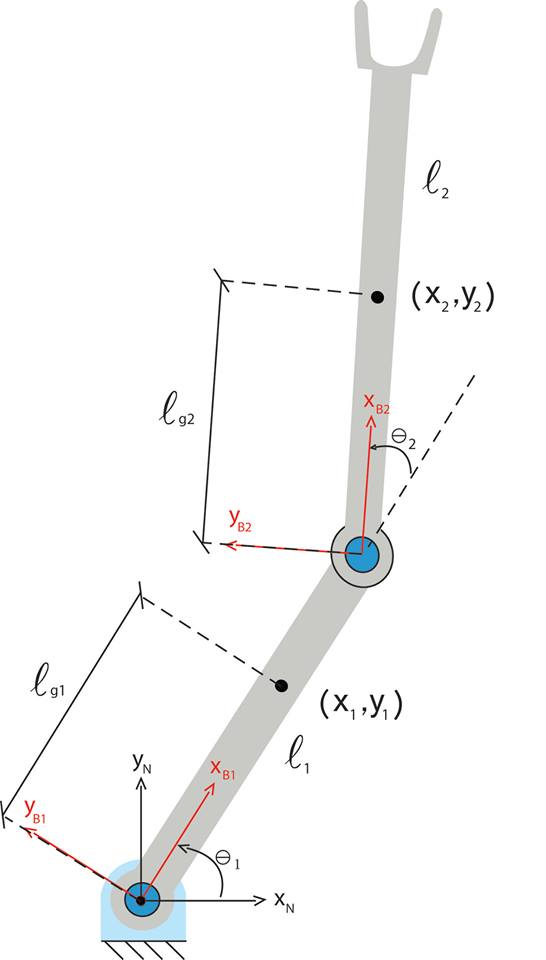
\includegraphics[scale=0.3]{RR.jpg}  
	\caption{Mecanismo \underline{R}\underline{R}}
	\label{fig:RR}
\end{figure}

\begin{itemize}
\item[1)] Defini\c{c}\~ao das coordenadas generalizadas:

\begin{equation}
\mq\ssh = \begin{bmatrix}
\theta_1 & \theta_2
\end{bmatrix}
\end{equation}
\begin{equation}
\mq\cir = \begin{bmatrix}
x_1 & y_1 & x_2 & y_2
\end{bmatrix}
\end{equation}

\item[2)] Defini\c{c}\~ao das velocidades generalizadas:

\begin{equation}
\mp\ssh = \begin{bmatrix}
\dot{\theta}_1 & \dot{\theta}_2
\end{bmatrix}
\end{equation}
\begin{equation}
\mp\cir = \begin{bmatrix}
\omega_{z1} & \omega_{z2} & v_{x1} & v_{y1} & v_{x2} & v_{y2}
\end{bmatrix}
\end{equation}

\item[3)] Cinem\'atica de posi\c{c}\~ao dos centros de massa e do efetuador utilizando matrizes de transforma\c{c}\~ao homog\^enea:

\begin{equation}
\hvct{\ttg_1}_{\ttB_1}  =
\begin{bmatrix} 
l_{g1} & 0 & 0 & 1
\end{bmatrix}^\msT
\end{equation}
\begin{equation}
\hvct{\ttg_2}_{\ttB_2}  =
\begin{bmatrix} 
l_{g2} & 0 & 0 & 1
\end{bmatrix}^\msT
\end{equation}
\begin{equation}
\hvct{\ttx}_{\ttB_2}  =
\begin{bmatrix} 
l_2 & 0 & 0 & 1
\end{bmatrix}^\msT
\end{equation}
\begin{equation}
\hvct{\mone}_{\ttN \rl \ttB_1} =
\begin{bmatrix}
\ccos_1 & -\ssin_1 & 0 & 0 \\
\ssin_1 & \ccos_1 & 0 & 0 \\
0 & 0 & 1 & 0 \\
0 & 0 & 0 & 1
\end{bmatrix}
\end{equation}
\begin{equation}
\hvct{\mone}_{\ttB_1 \rl \ttB_2} =
\begin{bmatrix}
\ccos_2 & -\ssin_2 & 0 & l_1 \\
\ssin_2 & \ccos_2 & 0 &  0 \\
0 & 0 & 1 & 0\\
0 & 0 & 0 & 1
\end{bmatrix}
\end{equation}
\begin{equation}
\hvct{\mone}_{\ttN \rl \ttB_2} = \hvct{\mone}_{\ttN \rl \ttB_1} \hvct{\mone}_{\ttB_1 \rl \ttB_2} =
\begin{bmatrix}
\ccos_{1\plus 2} & -\ssin_{1\plus 2} & 0 & l_1 \ccos_1\\
\ssin_{1\plus 2} & \ccos_{1\plus 2} & 0 & l_1 \ssin_1 \\
0 & 0 & 1 & 0\\
0 & 0 & 0 & 1
\end{bmatrix}
\end{equation}
\begin{equation}
\hvct{\ttg_1}_{\ttN}  = \hvct{\mone}_{\ttN \rl \ttB_1} \hvct{\ttg_1}_{\ttB_1} =
\begin{bmatrix}
l_{g1} \ccos_1 \\
l_{g1} \ssin_1 \\
0 \\
1
\end{bmatrix}
\end{equation}
\begin{equation}
\hvct{\ttg_2}_{\ttN}  = \hvct{\mone}_{\ttN \rl \ttB_2} \hvct{\ttg_2}_{\ttB_2} =
\begin{bmatrix}
l_1 \ccos_1 + l_{g2} \ccos_{1\plus 2} \\
l_1 \ssin_1 + l_{g2} \ssin_{1\plus 2} \\
0 \\
1
\end{bmatrix}
\end{equation}
\begin{equation}
\hvct{\ttx}_{\ttN}  = \hvct{\mone}_{\ttN \rl \ttB_2} \hvct{\ttx}_{\ttB_2} =
\begin{bmatrix}
l_1 \ccos_1 + l_2 \ccos_{1\plus 2} \\
l_1 \ssin_1 + l_2 \ssin_{1\plus 2} \\
0 \\
1
\end{bmatrix}
\end{equation}

\item[4)] Cinem\'atica de velocidades dos centros de massa:

\begin{equation}
[\underline{\vv}_1]_{\ttN} = \frac{\dd}{\dd t} [\ttg_1]_\ttN =
\begin{bmatrix}
-l_{g1} \ssin_1 \dot{\theta}_1 \\
 l_{g1} \ccos_1 \dot{\theta}_1 \\
 0 \\
\end{bmatrix}
\end{equation}
\begin{equation}
[\underline{\vv}_2]_{\ttN} = \frac{\dd}{\dd t} [\ttg_2]_\ttN =
\begin{bmatrix}
-l_{1} \ssin_1 \dot{\theta}_1 - l_{g2} \ssin_{1\plus 2} ( \dot{\theta}_1 + \dot{\theta}_2 )\\
 l_{1} \ccos_1 \dot{\theta}_1 + l_{g2} \ccos_{1\plus 2} ( \dot{\theta}_1 + \dot{\theta}_2 )\\
 0 \\
\end{bmatrix}
\end{equation}

\item[5)] Cinem\'atica de velocidades angulares das barras:

\begin{equation}
\smat{\underline{\vomega}_1}_{\ttB_1 \rl \ttB_1} = \tvct{\mone}_{\ttN \rl \ttB_1} \frac{\dd}{\dd t} \vct{\mone}_{\ttN \rl \ttB_1} = 
\begin{bmatrix}
0 & -\dot{\theta}_1 & 0 \\
\dot{\theta}_1 & 0 & 0 \\
0 & 0 & 0
\end{bmatrix}
\Rightarrow
\vct{\underline{\vomega}_1}_{\ttB_1} = 
\begin{bmatrix}
0 \\
0 \\
\dot{\theta}_1
\end{bmatrix}
\end{equation}
\begin{equation}
\smat{\underline{\vomega}_2}_{\ttB_2 \rl \ttB_2} = \tvct{\mone}_{\ttN \rl \ttB_2} \frac{\dd}{\dd t} \vct{\mone}_{\ttN \rl \ttB_2} = 
\begin{bmatrix}
0 & -\dot{\theta}_1 -\dot{\theta}_2 & 0 \\
\dot{\theta}_1 + \dot{\theta}_2 & 0 & 0 \\
0 & 0 & 0
\end{bmatrix}
\Rightarrow
\vct{\underline{\vomega}_2}_{\ttB_2} = 
\begin{bmatrix}
0 \\
0 \\
\dot{\theta}_1 + \dot{\theta}_2
\end{bmatrix}
\end{equation}

\item[6)] Montar o vetor $\underline{\mp}\cir(\mq\ssh,\mp\ssh)$ e calcular $\mC$, $\mA$ e $\mb$ atrav\'es das equa\c{c}\~oes \eqref{eq:MatrizC}, \eqref{eq:MatrizA} e \eqref{eq:Matrizb}:

\begin{equation}
\underline{\mp}\cir(\mq\ssh,\mp\ssh) =
\begin{bmatrix}
\dot{\theta}_1 \\
\dot{\theta}_1 + \dot{\theta}_2 \\
-l_{g1} \ssin_1 \dot{\theta}_1 \\
 l_{g1} \ccos_1 \dot{\theta}_1 \\
 -l_{1} \ssin_1 \dot{\theta}_1 - l_{g2} \ssin_{1\plus 2} ( \dot{\theta}_1 + \dot{\theta}_2 )\\
 l_{1} \ccos_1 \dot{\theta}_1 + l_{g2} \ccos_{1\plus 2} ( \dot{\theta}_1 + \dot{\theta}_2 )\\
\end{bmatrix}
\end{equation}
\begin{equation}
\frac{\partial \underline{\mp}\cir}{\partial \mp\ssh} =
\begin{bmatrix}
1 & 0 \\
1 & 1 \\
-l_{g1} \ssin_1 & 0 \\
 l_{g1} \ccos_1 & 0 \\
-l_{1} \ssin_1  - l_{g2} \ssin_{1\plus 2} & - l_{g2} \ssin_{1\plus 2} \\
 l_{1} \ssin_1  + l_{g2} \ccos_{1\plus 2} &   l_{g2} \ccos_{1\plus 2} \\
\end{bmatrix}
\end{equation}

\begin{equation}
\mC =
\begin{bmatrix}
1 & 0 \\
0 & 1 \\
1 & 0 \\
1 & 1 \\
-l_{g1} \ssin_1 & 0 \\
 l_{g1} \ccos_1 & 0 \\
-l_{1} \ssin_1  - l_{g2} \ssin_{1\plus 2} & - l_{g2} \ssin_{1\plus 2} \\
 l_{1} \ssin_1  + l_{g2} \ccos_{1\plus 2} &   l_{g2} \ccos_{1\plus 2} \\
\end{bmatrix}
\end{equation}
\begin{equation}
\mA =
\begin{bmatrix}
1 & 0 & -1 & 0 & 0 & 0 & 0 & 0 \\
1 & 1 & 0 & -1 & 0 & 0 & 0 & 0 \\
-l_{g1} \ssin_1 & 0 & 0 & 0 & -1 & 0 & 0 & 0 \\
 l_{g1} \ccos_1 & 0 & 0 & 0 & 0 & -1 & 0 & 0 \\
-l_{1} \ssin_1  - l_{g2} \ssin_{1\plus 2} & - l_{g2} \ssin_{1\plus 2} & 0 & 0 & 0 & 0 & -1 & 0 \\
 l_{1} \ccos_1  + l_{g2} \ccos_{1\plus 2} &   l_{g2} \ccos_{1\plus 2} & 0 & 0 & 0 & 0 & 0 & -1 \\
\end{bmatrix}
\end{equation}

\begin{equation}
\mb =
\begin{bmatrix}
0 \\
0 \\
l_{g1} \ccos_1 \dot{\theta}_1^2 \\
l_{g1} \ssin_1 \dot{\theta}_1^2 \\
l_{1} \ccos_1 \dot{\theta}_1^2  + l_{g2} \ccos_{1\plus 2}  (\dot{\theta}_1+\dot{\theta}_2)^2 \\
l_{1} \ssin_1  \dot{\theta}_1^2 + l_{g2} \ssin_{1\plus 2}   (\dot{\theta}_1+\dot{\theta}_2)^2 \\
\end{bmatrix}
\end{equation}

\item[7)] Calcular a energia de acelera\c{c}\~oes $S$:

\begin{equation}
S = \frac{1}{2} \Big( m_1 (\dot{v}_{x1}^2 + \dot{v}_{y1}^2) + m_2 (\dot{v}_{x2}^2 + \dot{v}_{y2}^2) + J_{z1} \dot{\omega}_{z1}^2 + + J_{z2} \dot{\omega}_{z2}^2 \Big)
\end{equation}

\item[8)] Obter $\mM$ e $\mv$ utilizando as equa\c{c}\~oes \eqref{eq:MatrizM} e \eqref{eq:Matrizv}:

\begin{equation}
\mM = \begin{bmatrix}
0 & 0 & J_{z1} & J_{z2} & m_1 & m_1 & m_2 & m_2
\end{bmatrix}^\msD
\end{equation}
\begin{equation}
\mv = \mzr
\end{equation}

\item[9)] Montar os vetores $\mf$, $\mg$ e $\mu$:

\begin{equation}
\mf =
\begin{bmatrix}
c_1 \dot{\theta}_1 + \gamma_1 \sign (\dot{\theta}_1) \\
c_2 \dot{\theta}_2 + \gamma_2 \sign (\dot{\theta}_2) \\
0 \\
0 \\
0 \\
0 \\
0 \\
0 \\
\end{bmatrix}
\end{equation}
\begin{equation}
\mg =
\begin{bmatrix}
0 \\
0 \\
0 \\
0 \\
0 \\
m_1 g \\
0 \\
m_2 g
\end{bmatrix}
\end{equation}
\begin{equation}
\mu =
\begin{bmatrix}
\tau_1 \\
\tau_2
\end{bmatrix}
\end{equation}

\end{itemize}

Sendo assim, a partir da equa\c{c}\~ao \eqref{eq:DinamicaDireta}, temos que o modelo para simula\c{c}\~ao din\^amica direta do mecanismo \underline{R}\underline{R} \'e dado por:

\small\begin{equation} \label{eq:RR}
\begin{cases}
\begin{bmatrix}
1 & 0 \\
0 & 1 \\
1 & 0 \\
1 & 1 \\
-l_{g1} \ssin_1 & 0 \\
 l_{g1} \ccos_1 & 0 \\
-l_{1} \ssin_1  - l_{g2} \ssin_{1\plus 2} & - l_{g2} \ssin_{1\plus 2} \\
 l_{1} \ssin_1  + l_{g2} \ccos_{1\plus 2} &   l_{g2} \ccos_{1\plus 2} \\
\end{bmatrix}^\msT
\begin{Bmatrix}
\begin{bmatrix}
0 \\ 0 \\ J_{z1} \\ J_{z2} \\ m_1 \\ m_1 \\ m_2 \\ m_2
\end{bmatrix}^\msD
\begin{bmatrix}
\ddot{\theta}_1 \\
\ddot{\theta}_2 \\
\dot{\omega}_{z1} \\
\dot{\omega}_{z2} \\
\dot{v}_{x1} \\
\dot{v}_{y1} \\
\dot{v}_{x2} \\
\dot{v}_{y2} \\
\end{bmatrix}
+
\begin{bmatrix}
c_1 \dot{\theta}_1 + \gamma_1 \sign (\dot{\theta}_1) \\
c_2 \dot{\theta}_2 + \gamma_2 \sign (\dot{\theta}_2) \\
0 \\
0 \\
0 \\
0 \\
0 \\
0 \\
\end{bmatrix}
+
\begin{bmatrix}
0 \\
0 \\
0 \\
0 \\
0 \\
m_1 g \\
0 \\
m_2 g
\end{bmatrix}
\end{Bmatrix}
=
\begin{bmatrix}
\tau_1 \\ \tau_2
\end{bmatrix} \\
\begin{bmatrix}
1 & 0 & -1 & 0 & 0 & 0 & 0 & 0 \\
1 & 1 & 0 & -1 & 0 & 0 & 0 & 0 \\
-l_{g1} \ssin_1 & 0 & 0 & 0 & -1 & 0 & 0 & 0 \\
 l_{g1} \ccos_1 & 0 & 0 & 0 & 0 & -1 & 0 & 0 \\
-l_{1} \ssin_1  - l_{g2} \ssin_{1\plus 2} & - l_{g2} \ssin_{1\plus 2} & 0 & 0 & 0 & 0 & -1 & 0 \\
 l_{1} \ccos_1  + l_{g2} \ccos_{1\plus 2} &   l_{g2} \ccos_{1\plus 2} & 0 & 0 & 0 & 0 & 0 & -1 \\
\end{bmatrix}
\begin{bmatrix}
\ddot{\theta}_1 \\
\ddot{\theta}_2 \\
\dot{\omega}_{z1} \\
\dot{\omega}_{z2} \\
\dot{v}_{x1} \\
\dot{v}_{y1} \\
\dot{v}_{x2} \\
\dot{v}_{y2} \\
\end{bmatrix} = 
\begin{bmatrix}
0 \\
0 \\
l_{g1} \ccos_1 \dot{\theta}_1^2 \\
l_{g1} \ssin_1 \dot{\theta}_1^2 \\
l_{1} \ccos_1 \dot{\theta}_1^2  + l_{g2} \ccos_{1\plus 2}  (\dot{\theta}_1+\dot{\theta}_2)^2 \\
l_{1} \ssin_1  \dot{\theta}_1^2 + l_{g2} \ssin_{1\plus 2}   (\dot{\theta}_1+\dot{\theta}_2)^2 \\
\end{bmatrix}
\end{cases}
\end{equation}\normalsize

\subsection{Algoritmo para modelagem de mecanismos paralelos}\label{S04-2}

Para realizar a modelagem de mecanismos paralelos a partir de subsistemas seriais j\'a deduzidos, \'e necess\'ario introduzir mais alguns conceitos: \\

Sejam $\ssB_0$, $\ssB_1$, ..., $\ssB_{n} \,$ $n+1$ subsistemas mec\^anicos e $\ssM$ um sistema mec\^anico de $\nu\ssh$ graus de liberdade gerado pelo acoplamento dos subsistemas citados. Definimos:

\begin{itemize}
\item $\mq_r$: matriz-coluna de coordenadas generalizadas que descrevem a orienta\c{c}\~ao da plataforma/efetuador $\ssB_0$. Normalmente \'e dada pelas componentes de um quaternion unit\'ario, i.e. $\mq_r = \begin{bmatrix} q_i & q_j & q_k & q_r \end{bmatrix}^\msT $ com $ \mq_r^\msT \cdot \mq_r = \vct{1}$.
\item $\mq_t$: matriz-coluna de coordenadas generalizadas que descrevem a posi\c{c}\~ao da plataforma/efetuador $\ssB_0$.
\item $\mq_0$: matriz-coluna de todas as coordenadas generalizadas da plataforma/efetuador $\ssB_0$. \'E definida como $\mq_0 = \begin{bmatrix} \mq_r^\msT & \mq_t^\msT \end{bmatrix}^\msT$.
\item $\mq_j\ssh, \,j=1, ..., n$: matriz-coluna de coordenadas generalizadas independentes do subsistema  $\ssB_j$.
\item $\mq\hcir$: matriz-coluna de coordenadas generalizadas redundantes n\~ao pertencentes \`a plataforma/efetuador. Definida como $\mq\hcir = \begin{bmatrix}  {\mq_1\ssh}^\msT & ... & {\mq_{n}\ssh}^\msT \end{bmatrix}^\msT $.
\item $\mq$: matriz-coluna contendo todas as coordenadas generalizadas do sistema $\ssM$. Definida como $\mq = \begin{bmatrix} \mq_0^\msT & {\mq\hcir}^\msT \end{bmatrix}^\msT $.
\item $\overline{\mq}(\mq)$: matriz-coluna dos v\'inculos de posi\c{c}\~ao entre subsistemas. As equa\c{c}\~oes vinculares s\~ao dadas por $\overline{\mq}(\mq) = \mzr $.
\item $\mp_r$: matriz-coluna de velocidades generalizadas associadas a movimentos de rota\c{c}\~ao (instant\^anea) em torno do centro de massa da plataforma/efetuador $\ssB_0$. Respeita $\mp_r = \mD(\mq_r)\dot{\mq}_r$, sendo $\mD(\mq_r)$ uma matriz de posto completo com n\'umero de colunas maior ou igual ou n\'umero de linhas tal que $\dot{\mq}_r  = \mD^\msP(\mq_r) \mp_r$.
\item $\mp_t$: matriz-coluna de velocidades generalizadas associadas \`a transla\c{c}\~ao do centro de massa de $\ssB_0$. \'E dada por $\mp_t = \dot{\mq}_t$.
\item $\mp\ssh_0$: matriz-coluna de todas as velocidades generalizadas independentes da plataforma/efetuador $\ssB_0$. \'E definida como $\mp\ssh_0 = \begin{bmatrix} \mp_r^\msT & \mp_t^\msT \end{bmatrix}^\msT$.
\item $\mp\cir_0$: matriz-coluna de velocidades generalizadas redundantes da plataforma/efetuador $\ssB_0$. \'E dada por $\mp\cir_0 = \dot{\mq}_r$.
\item $\mp_j\ssh, \,j=1, ..., n$: matriz-coluna de velocidades generalizadas independentes do subsistema  $\ssB_j$. \'E definida por $\mp_j\ssh = \dot{\mq}_j\ssh$.
\item $\mp_j\cir, \,j=1, ..., n$: matriz-coluna de velocidades generalizadas redundantes do subsistema  $\ssB_j$.
\item $\mp_j, \,j=0, ..., n$: matriz-coluna de velocidades generalizadas do subsistema  $\ssB_j$. \'E definida por $\mp_j = \begin{bmatrix} {\mp_j\ssh}^\msT & {\mp_j\cir}^\msT \end{bmatrix}$.
\item $\mp\ssh$: matriz-coluna de $\nu\ssh$ velocidades generalizadas independentes de $\ssM$. \'E dada por $\mp\ssh = \mp_0\ssh$.
\item $\mp\cir$: matriz-coluna de velocidades generalizadas redundantes de $\ssM$. \'E definida por $\mp\cir = \begin{bmatrix} {\mp\cir_0}^\msT & \mp_1^\msT & ... & \mp_{n}^\msT \end{bmatrix}^\msT $.
\item $\mp$: matriz-coluna contendo todas as velocidades generalizadas de $\ssM$. \'E definida por $\mp = \begin{bmatrix} {\mp\ssh}^\msT & {\mp\cir}^\msT \end{bmatrix}^\msT $.
\item $\mrho$: matriz-coluna definida como $\mrho = \begin{bmatrix} {\mrho\ssh}^\msT & {\mrho\cir}^\msT \end{bmatrix}^\msT $, sendo $\mrho\ssh = \mp_0\ssh$ e $\mrho\cir = \dot{\mq}\hcir = \begin{bmatrix} {\mp\ssh_1}^\msT & ... &  {\mp\ssh_n}^\msT \end{bmatrix}^\msT $.
\item $\underline{\dot{\mq}}(\mq,\mrho)$: $\dot{\mq}$ escrita em fun\c{c}\~ao de $\mq$ e $\mrho$.
\item $\overline{\momega}(\mq,\mrho)$: matriz-coluna dos v\'inculos de orienta\c{c}\~ao entre subsistemas. As equa\c{c}\~oes vinculares s\~ao dadas por $\overline{\momega}(\mq,\mrho) = \mzr $.
\item $\overline{\mrho}(\mq,\mrho)$: matriz-coluna de todos os v\'inculos de velocidades entre subsistemas. As equa\c{c}\~oes vinculares s\~ao dadas por $\overline{\mrho}(\mq,\mrho) = \mzr $.
\item $\mA_j(\mq), \,j=0, ..., n$: Jacobiano dos v\'inculos de velocidades do subsistema $\ssB_j$.
\item $\mC_j(\mq), \,j=0, ..., n$: complemento ortogonal do Jacobiano dos v\'inculos de velocidades do subsistema $\ssB_j$.
\item $\mM_j, \,j=0, ..., n$: matriz de in\'ercia desacoplada do subsistema $\ssB_j$.
\item $\mv_j(\mp), \,j=0, ..., n$: matriz-coluna dos termos girosc\'opicos desacoplados do subsistema $\ssB_j$.
\item $\mf_j(\mq), \,j=0, ..., n$: matriz-coluna dos esfor\c{c}os de atrito do subsistema $\ssB_j$.
\item $\mg_j, \,j=0, ..., n$: matriz-coluna dos esfor\c{c}os gravitacionais do subsistema $\ssB_j$.
\item $\mu_j, \,j=0, ..., n$: matriz-coluna dos esfor\c{c}os ativos externos do subsistema $\ssB_j$.
\end{itemize}

O modelo para simula\c{c}\~ao din\^amica direta \'e dado pelo seguinte equacionamento:
\begin{equation} \label{eq:DinamicaDireta2}
\begin{cases}
\mC^\msT(\mq) \Big( \mM \dot{\mp} + \mv(\mp) + \mf(\mp) + \mg \Big) = \breve{\mC}^\msT(\mq) \mu \\
\mA(\mq) \dot{\mp} = \mb(\mq,\mp)
\end{cases}
\end{equation}
Sendo:
\begin{equation} \label{eq:dq}
\underline{\dot{\mq}}(\mq,\mrho) = \begin{bmatrix}
\mD^\msP \mp_r \\
\mp_t \\
\mp\ssh_1 \\
\vdots \\
\mp\ssh_n \\
\end{bmatrix}
=
\begin{bmatrix}
\mD^\msP  & \mzr & \mzr & \ldots & \mzr\\
\mzr & \mone & \mzr & \ldots & \mzr\\
\mzr & \mzr & \mone & \ldots & \mzr\\
\vdots & \vdots & \vdots &  \ddots & \vdots\\
\mzr  & \mzr & \mzr &\ldots & \mone
\end{bmatrix}
\begin{bmatrix}
\mp_r \\
\mp_t \\
\mp\ssh_1 \\
\vdots \\
\mp\ssh_n \\
\end{bmatrix}
=
\begin{bmatrix}
\mD^\msP  & \mzr & \mzr & \ldots & \mzr\\
\mzr & \mone & \mzr & \ldots & \mzr\\
\mzr & \mzr & \mone & \ldots & \mzr\\
\vdots & \vdots & \vdots &  \ddots & \vdots\\
\mzr  & \mzr & \mzr &\ldots & \mone
\end{bmatrix}
\mrho
\end{equation}
\begin{equation} \label{eq:VinculosVelocidades}
\overline{\mrho} = \begin{bmatrix}
\displaystyle\frac{\partial \overline{\mq}}{\partial \mq} \cdot \underline{\dot{\mq}} \\
\overline{\momega}
\end{bmatrix}
\end{equation}
\begin{equation} \label{eq:MatrizCchapeu}
\breve{\mC} = \begin{bmatrix}
\mone \\
- \displaystyle\frac{\partial \overline{\mrho}}{\partial \mrho\cir}^\msP \frac{\partial \overline{\mrho}}{\partial \mrho\ssh }
\end{bmatrix}
\end{equation}
\begin{equation} \label{eq:MatrizC2}
\mC = 
\begin{bmatrix}
\mC_0 &  \mzr  & \ldots & \mzr\\
\mzr  &  \mC_1 & \ldots & \mzr\\
\vdots & \vdots & \ddots & \vdots\\
\mzr  &   \mzr       &\ldots & \mC_{n}
\end{bmatrix}
\breve{\mC}
\end{equation}
\begin{equation} \label{eq:MatrizA2}
\mA = 
\begin{bmatrix}
\begin{bmatrix}
\mA_0  & \mzr & \ldots & \mzr\\
\mzr & \mA_1 & \ldots & \mzr\\
\vdots & \vdots & \ddots & \vdots\\
\mzr  & \mzr     &\ldots & \mA_{n}
\end{bmatrix} \\
\displaystyle\frac{\partial \overline{\mrho}}{\partial \mp}
\end{bmatrix}
\end{equation}
\begin{equation} \label{eq:Matrizb2}
\mb = - \dot{\mA}(\mq,\mp) \mp
\end{equation}
\begin{equation} \label{eq:MatrizM2}
\mM =
\begin{bmatrix}
\mM_0 &  \mzr  & \ldots & \mzr\\
\mzr  &  \mM_1 & \ldots & \mzr\\
\vdots & \vdots & \ddots & \vdots\\
\mzr  &   \mzr       &\ldots & \mM_{n}
\end{bmatrix}
\end{equation}
\begin{equation} \label{eq:Matrizv2}
\mv = \begin{bmatrix}
\mv_0^\msT & \mv_1^\msT & ... & \mv_{n}^\msT
\end{bmatrix}^\msT
\end{equation}
\begin{equation} \label{eq:Matrizf2}
\mf = \begin{bmatrix}
\mf_0^\msT & \mf_1^\msT & ... & \mf_{n}^\msT
\end{bmatrix}^\msT
\end{equation}
\begin{equation} \label{eq:Matrizg2}
\mg = \begin{bmatrix}
\mg_0^\msT & \mg_1^\msT & ... & \mg_{n}^\msT
\end{bmatrix}^\msT
\end{equation}
\begin{equation}
\mu =
\begin{bmatrix} \label{eq:Matrizu}
\mu_0^\msT & \mu_1^\msT & ... & \mu_{n}^\msT
\end{bmatrix}^\msT
\end{equation}

Aqui seguem as etapas do algoritmo para dedu\c{c}\~ao do modelo din\^amico de um mecanismo paralelo acompanhado de um exemplo de aplica\c{c}\~ao, a dedu\c{c}\~ao do modelo din\^amico do mecanismo 5R (pent\'agono articulado) a partir do acoplamento dos modelos de 2 mecanismos \underline{R}\underline{R} e uma massa pontual (efetuador).

\begin{figure}[H]
	\centering
	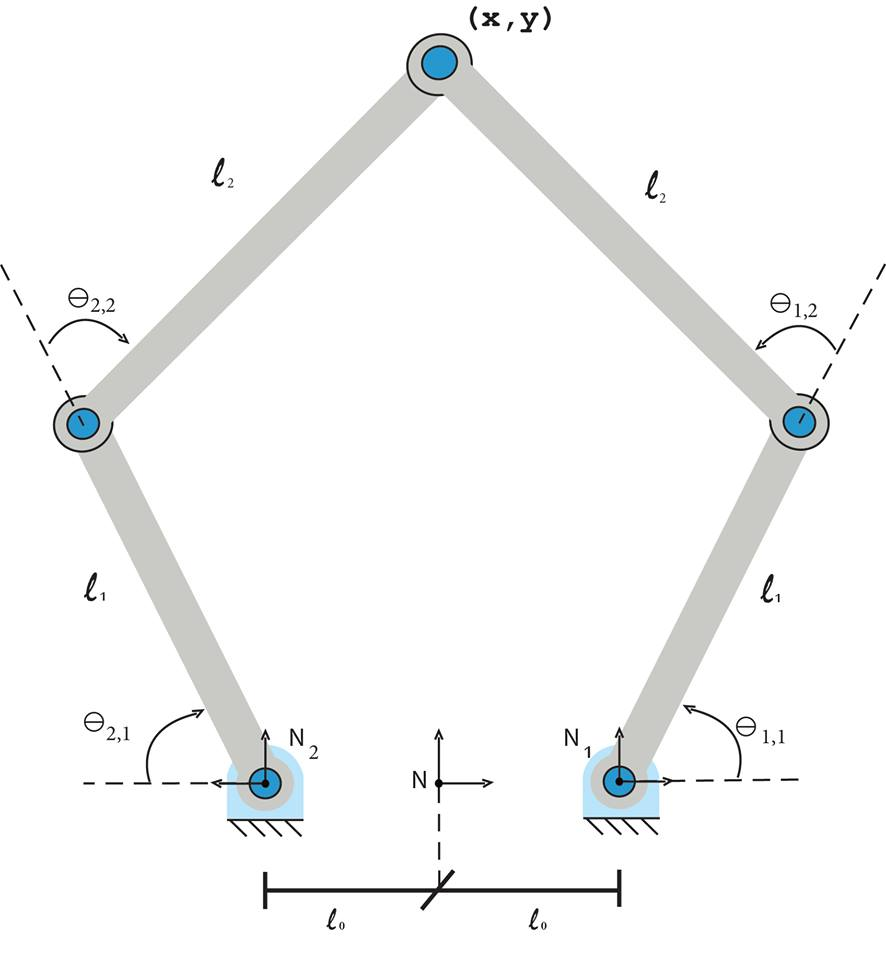
\includegraphics[scale=0.4]{5Rscan.jpg}
	\caption{Mecanismo 5R}
	\label{fig:RR}
\end{figure}

O modelo do mecanismo \underline{R}\underline{R} \'e dado pela equa\c{c}\~ao \eqref{eq:RR}. O modelo da massa pontual \'e dado pela seguinte express\~ao:
\begin{equation} \label{eq:MassaPontual}
\begin{bmatrix}
m_0 \\
m_0 \\
\end{bmatrix}^\msD
\begin{bmatrix}
\ddot{x} \\
\ddot{y}
\end{bmatrix}
+
\begin{bmatrix}
0 \\
m_0 g
\end{bmatrix}
=
\begin{bmatrix}
0 \\
0
\end{bmatrix}
\end{equation}

Etapas do algoritmo:

\begin{itemize}
\item[1)] Defini\c{c}\~ao das coordenadas generalizadas:

\begin{equation}
\mq_r = \vct{\varnothing}
\end{equation}

\begin{equation}
\mq_t = \begin{bmatrix}
x & y
\end{bmatrix}^\msT
\end{equation}
\begin{equation}
\mq_1\ssh = \begin{bmatrix}
\theta_{1,1} &
\theta_{1,2} 
\end{bmatrix}^\msT
\end{equation}
\begin{equation}
\mq_2\ssh = \begin{bmatrix}
\theta_{2,1} &
\theta_{2,2}
\end{bmatrix}^\msT
\end{equation}

\item[2)] Defini\c{c}\~ao das velocidades generalizadas:

\begin{equation}
\mp_r = \vct{\varnothing}
\end{equation}
\begin{equation}
\mp_t = \dot{\mq}_t = 
\begin{bmatrix}
\dot{x} & \dot{y}
\end{bmatrix}^\msT
\end{equation}
\begin{equation}
\mp_1\cir = \begin{bmatrix}
\omega_{1,z1} & \omega_{1,z2} & v_{1,x1} & v_{1,y1} & v_{1,x2} & v_{1,y2}
\end{bmatrix}^\msT
\end{equation}
\begin{equation}
\mp_2\cir = \begin{bmatrix}
\omega_{2,z1} & \omega_{2,z2} & v_{2,x1} & v_{2,y1} & v_{2,x2} & v_{2,y2}
\end{bmatrix}^\msT
\end{equation}

\item[3)] Defini\c{c}\~ao dos v\'inculos de posi\c{c}\~ao entre subsistemas utilizando matrizes de transforma\c{c}\~ao homog\^enea:

\begin{equation}
\hvct{\mone}_{\ttN \rl \ttN_1} =
\begin{bmatrix}
1 & 0 & 0 & l_0 \\
0 & 1 & 0 & 0 \\
0 & 0 & 1 & 0 \\
0 & 0 & 0 & 1
\end{bmatrix}
\end{equation}
\begin{equation}
\hvct{\mone}_{\ttN \rl \ttN_2} =
\begin{bmatrix}
-1 & 0 & 0 & -l_0 \\
0 & 1 & 0 & 0 \\
0 & 0 & -1 & 0\\
0 & 0 & 0 & 1
\end{bmatrix}
\end{equation}
\begin{equation}
\vct{\ttx_0}_{\ttN} =
\begin{bmatrix}
x \\
y \\
0 \\
\end{bmatrix}
\end{equation}
\begin{equation}
\vct{\ttx_1}_{\ttN_1} =
\begin{bmatrix}
l_1 \ccos_{1,1} + l_2 \ccos_{1,1\plus 2} \\
l_1 \ssin_{1,1} + l_2 \ssin_{1,1\plus 2} \\
0
\end{bmatrix}
\end{equation}
\begin{equation}
\vct{\ttx_2}_{\ttN_2} =
\begin{bmatrix}
l_1 \ccos_{2,1} + l_2 \ccos_{2,1\plus 2} \\
l_1 \ssin_{2,1} + l_2 \ssin_{2,1\plus 2} \\
0
\end{bmatrix}
\end{equation}
\begin{equation}
\hvct{\ttx_1}_{\ttN} = \hvct{\mone}_{\ttN \rl \ttN_1} \hvct{\ttx_1}_{\ttN_1} =
\begin{bmatrix}
l_0 + l_1 \ccos_{1,1} + l_2 \ccos_{1,1\plus 2} \\
l_1 \ssin_{1,1} + l_2 \ssin_{1,1\plus 2} \\
0 \\
1
\end{bmatrix}
\end{equation}
\begin{equation}
\hvct{\ttx_2}_{\ttN} = \hvct{\mone}_{\ttN \rl \ttN_2} \hvct{\ttx_2}_{\ttN_2} =
\begin{bmatrix}
-l_0 - l_1 \ccos_{2,1} - l_2 \ccos_{2,1\plus 2} \\
l_1 \ssin_{2,1} + l_2 \ssin_{2,1\plus 2} \\
0 \\
1
\end{bmatrix}
\end{equation}

V\'inculos de posi\c{c}\~ao:

\begin{equation}
\begin{cases}
\vct{\ttx_0}_{\ttN} = \vct{\ttx_1}_{\ttN} \\
\vct{\ttx_0}_{\ttN} = \vct{\ttx_2}_{\ttN} \\
\end{cases}
\Rightarrow
\begin{cases}
x = l_0 + l_1 \ccos_{1,1} + l_2 \ccos_{1,1\plus 2} \\
y = l_1 \ssin_{1,1} + l_2 \ssin_{1,1\plus 2} \\ 
x = -l_0 - l_1 \ccos_{2,1} - l_2 \ccos_{2,1\plus 2} \\
y = l_1 \ssin_{2,1} + l_2 \ssin_{2,1\plus 2} \\
\end{cases}
\end{equation}
\begin{equation}
\therefore \overline{\mq}(\mq) = 
\begin{bmatrix}
x - l_0 - l_1 \ccos_{1,1} - l_2 \ccos_{1,1\plus 2} \\
y - l_1 \ssin_{1,1} - l_2 \ssin_{1,1\plus 2} \\
x + l_0 + l_1 \ccos_{2,1} + l_2 \ccos_{2,1\plus 2} \\
y - l_1 \ssin_{2,1} - l_2 \ssin_{2,1\plus 2} \\
\end{bmatrix}
= \mzr
\end{equation}

\item[4)] Defini\c{c}\~ao dos v\'inculos de orienta\c{c}\~ao entre subsistemas:
\begin{equation}
\overline{\momega}(\mq,\mrho) = \vct{\varnothing}
\end{equation}

Nesse exemplo n\~ao h\'a v\'inculos de orienta\c{c}\~ao entre subsistemas.

\item[5)] C\'alculo dos Jacobianos dos v\'inculos de posi\c{c}\~ao e defini\c{c}\~ao dos v\'inculos de velocidades atrav\'es de \eqref{eq:VinculosVelocidades}:

\begin{equation}
\frac{\partial \overline{\mq}}{\partial \mq} = 
\begin{bmatrix}
1 & 0 & l_1 \ssin_{1,1} + l_2 \ssin_{1\plus 2} &  l_2 \ssin_{1\plus 2} & 0 & 0 \\
0 & 1 & -l_1 \ccos_{1,1} - l_2 \ccos_{1\plus 2} & -l_2 \ccos_{1\plus 2} & 0 & 0  \\
1 & 0 & 0 & 0 & -l_1 \ssin_{2,1} - l_2 \ssin_{2\plus 2} & -l_2 \ssin_{2\plus 2}  \\
0 & 1 & 0 & 0 & -l_1 \ccos_{2,1} - l_2 \ccos_{2\plus 2} & -l_2 \ccos_{2\plus 2}   \\
\end{bmatrix}
\end{equation}
\begin{equation}
\underline{\dot{\mq}}(\mq,\mrho) = \begin{bmatrix}
\dot{x} &
\dot{y} &
\dot{\theta}_{1,1} &
\dot{\theta}_{1,2} &
\dot{\theta}_{2,1} &
\dot{\theta}_{2,2}
\end{bmatrix}^\msT
\end{equation}
\begin{equation}
\overline{\mrho}(\mq,\mrho) =  
\begin{bmatrix}
1 & 0 & l_1 \ssin_{1,1} + l_2 \ssin_{1\plus 2} &  l_2 \ssin_{1\plus 2} & 0 & 0 \\
0 & 1 & -l_1 \ccos_{1,1} - l_2 \ccos_{1\plus 2} & -l_2 \ccos_{1\plus 2} & 0 & 0  \\
1 & 0 & 0 & 0 & -l_1 \ssin_{2,1} - l_2 \ssin_{2\plus 2} & -l_2 \ssin_{2\plus 2}  \\
0 & 1 & 0 & 0 & -l_1 \ccos_{2,1} - l_2 \ccos_{2\plus 2} & -l_2 \ccos_{2\plus 2}   \\
\end{bmatrix}
\begin{bmatrix}
\dot{x} \\
\dot{y} \\
\dot{\theta}_{1,1} \\
\dot{\theta}_{1,2} \\
\dot{\theta}_{2,1} \\
\dot{\theta}_{2,2}
\end{bmatrix}
 = \mzr
\end{equation}

\item[6)] C\'alculo de $\breve{\mC}$, $\mC$, $\mA$ e $\mb$ atrav\'es de \eqref{eq:MatrizCchapeu}, \eqref{eq:MatrizC2}, \eqref{eq:MatrizA2} e \eqref{eq:Matrizb2}:

\begin{equation}
\breve{\mC} =
\begin{bmatrix}
1 & 0 \\
0 & 1 \\
\displaystyle\frac{\ccos_{1,1\plus 2}}{l_1 \ssin_{1,2}} & \displaystyle\frac{\ssin_{1,1\plus 2}}{l_1 \ssin_{1,2}} \\
-\displaystyle\frac{l_1\ccos_{1,1} + l_2\ccos_{1,1\plus 2}}{l_1 l_2 \ssin_{1,2}} & -\displaystyle\frac{l_1\ssin_{1,1} + l_2\ssin_{1,1\plus 2}}{l_1 l_2 \ssin_{1,2}} \\
-\displaystyle\frac{\ccos_{2,1\plus 2}}{l_1 \ssin_{2,2}} & \displaystyle\frac{\ssin_{2,1\plus 2}}{l_1 \ssin_{2,2}} \\
\displaystyle\frac{l_1\ccos_{2,1} + l_2\ccos_{2,1\plus 2}}{l_1 l_2 \ssin_{2,2}} & -\displaystyle\frac{l_1\ssin_{2,1} + l_2\ssin_{2,1\plus 2}}{l_1 l_2 \ssin_{2,2}} \\
\end{bmatrix}
\end{equation}

\footnotesize\begin{equation}
\mC =
\begin{bmatrix}
1 & 0 \\
0 & 1 \\
\displaystyle\frac{\ccos_{1,1\plus 2}}{l_1 s_{1,2}} & \displaystyle\frac{\ssin_{1,1\plus 2}}{l_1 s_{1,2}} \\
-\displaystyle\frac{l_1 \ccos_{1,1} + l_2 \ccos_{1,1\plus 2}}{l_1 l_2 \ssin_{1,2}} & -\displaystyle\frac{l_1 \ssin_{1,1} + l_2 \ssin_{1,1\plus 2}}{l_1 l_2 \ssin_{1,2}} \\
\displaystyle\frac{\ccos_{1,1\plus 2}}{l_1 s_{1,2}} & \displaystyle\frac{\ssin_{1,1\plus 2}}{l_1 s_{1,2}} \\
-\displaystyle\frac{\ccos_{\theta_{1,1}}}{l_2 s_{1,2}} & -\displaystyle\frac{\ssin_{\theta_{1,1}}}{l_2 s_{1,2}} \\
-\displaystyle\frac{l_{g1} \ssin_{1,1} \ccos_{1,1\plus 2}}{l_1 \ssin_{1,2}} & -\displaystyle\frac{l_{g1} \ssin_{1,1} \ssin_{1,1\plus 2}}{l_1 \ssin_{1,2}} \\
\displaystyle\frac{l_{g1} \ccos_{1,1} \ccos_{1,1\plus 2}}{l_1 \ssin_{1,2}} & \displaystyle\frac{l_{g1} \ccos_{1,1} \ssin_{1,1\plus 2}}{l_1 \ssin_{1,2}} \\
-\displaystyle\frac{l_2 \ssin_{1,1}\ccos_{1,1\plus 2} - l_{g2} \ccos_{1,1} \ssin_{1,1\plus 2} }{l_2 \ssin_{1,2}} & -\displaystyle\frac{(l_2 - l_{g2}) \ssin_{1,1}\ssin_{1,1\plus 2} }{l_2 \ssin_{1,2}} \\
\displaystyle\frac{(l_2 - l_{g2}) \ccos_{1,1}\ccos_{1,1\plus 2} }{l_2 \ssin_{1,2}} & -\displaystyle\frac{l_2 \ccos_{1,1}\ssin_{1,1\plus 2} - l_{g2} \ssin_{1,1} \ccos_{1,1\plus 2} }{l_2 \ssin_{1,2}} \\
-\displaystyle\frac{\ccos_{2,1\plus 2}}{l_1 s_{2,2}} & \displaystyle\frac{\ssin_{2,1\plus 2}}{l_1 s_{2,2}} \\
\displaystyle\frac{l_1 \ccos_{2,1} + l_2 \ccos_{2,1\plus 2}}{l_1 l_2 \ssin_{2,2}} & -\displaystyle\frac{l_1 \ssin_{2,1} + l_2 \ssin_{2,1\plus 2}}{l_1 l_2 \ssin_{2,2}} \\
-\displaystyle\frac{\ccos_{2,1\plus 2}}{l_1 s_{2,2}} & \displaystyle\frac{\ssin_{2,1\plus 2}}{l_1 s_{2,2}} \\
\displaystyle\frac{\ccos_{2,1}}{l_2 s_{2,2}} & -\displaystyle\frac{\ssin_{2,1}}{l_2 s_{2,2}} \\
\displaystyle\frac{l_{g1} \ssin_{2,1} \ccos_{2,1\plus 2}}{l_1 \ssin_{2,2}} & -\displaystyle\frac{l_{g1} \ssin_{2,1} \ssin_{2,1\plus 2}}{l_1 \ssin_{2,2}} \\
-\displaystyle\frac{l_{g1} \ccos_{2,1} \ccos_{2,1\plus 2}}{l_1 \ssin_{2,2}} & \displaystyle\frac{l_{g1} \ccos_{2,1} \ssin_{2,1\plus 2}}{l_1 \ssin_{2,2}} \\
\displaystyle\frac{l_2 \ssin_{2,1}\ccos_{2,1\plus 2} - l_{g2} \ccos_{2,1} \ssin_{2,1\plus 2} }{l_2 \ssin_{2,2}} & -\displaystyle\frac{(l_2 - l_{g2}) \ssin_{2,1}\ssin_{2,1\plus 2} }{l_2 \ssin_{2,2}} \\
\displaystyle\frac{(l_2 - l_{g2}) \ccos_{2,1}\ccos_{2,1\plus 2} }{l_2 \ssin_{2,2}} & -\displaystyle\frac{l_2 \ccos_{2,1}\ssin_{2,1\plus 2} - l_{g2} \ssin_{2,1} \ccos_{2,1\plus 2} }{l_2 \ssin_{2,2}} \\
\end{bmatrix}
\end{equation}\normalsize

\end{itemize}

\footnotesize\begin{equation}
\mA =\begin{bmatrix}
0 & 0 &1 & 0 & \mminus 1 & 0 & 0 & 0 & 0 & 0 & 0 & 0 & 0 & 0 & 0 & 0 & 0 & 0 \\
0 & 0 &1 & 1 & 0 & \mminus 1 & 0 & 0 & 0 & 0 & 0 & 0 & 0 & 0 & 0 & 0 & 0 & 0 \\
0 & 0 &\mminus l_{g1} \ssin_1 & 0 & 0 & 0 & \mminus 1 & 0 & 0 & 0 & 0 & 0 & 0 & 0 & 0 & 0 & 0 & 0 \\
0 & 0 & l_{g1} \ccos_1 & 0 & 0 & 0 & 0 & \mminus 1 & 0 & 0 & 0 & 0 & 0 & 0 & 0 & 0 & 0 & 0 \\
0 & 0 &\mminus l_{1} \ssin_1  \mminus  l_{g2} \ssin_{1\plus 2} & \mminus  l_{g2} \ssin_{1\plus 2} & 0 & 0 & 0 & 0 & \mminus 1 & 0  & 0 & 0 & 0 & 0 & 0 & 0 & 0 & 0 \\
0 & 0 & l_{1} \ccos_1  \pplus l_{g2} \ccos_{1\plus 2} &   l_{g2} \ccos_{1\plus 2} & 0 & 0 & 0 & 0 & 0 & \mminus 1 & 0 & 0 & 0 & 0 & 0 & 0 & 0 & 0 \\
0 & 0 & 0 & 0 & 0 & 0 & 0 & 0 & 0 & 0 & 1 & 0 & \mminus 1 & 0 & 0 & 0 & 0 & 0 \\
0 & 0 & 0 & 0 & 0 & 0 & 0 & 0 & 0 & 0 & 1 & 1 & 0 & \mminus 1 & 0 & 0 & 0 & 0 \\
0 & 0 & 0 & 0 & 0 & 0 & 0 & 0 & 0 & 0 & \mminus l_{g1} \ssin_1 & 0 & 0 & 0 & \mminus 1 & 0 & 0 & 0 \\
0 & 0 & 0 & 0 & 0 & 0 & 0 & 0 & 0 & 0 &  l_{g1} \ccos_1 & 0 & 0 & 0 & 0 & \mminus 1 & 0 & 0\\
0 & 0 & 0 & 0 & 0 & 0 & 0 & 0 & 0 & 0 & \mminus l_{1} \ssin_1  \mminus  l_{g2} \ssin_{1\plus 2} & \mminus  l_{g2} \ssin_{1\plus 2} & 0 & 0 & 0 & 0 & \mminus 1 & 0 \\
0 & 0 & 0 & 0 & 0 & 0 & 0 & 0 & 0 & 0 & l_{1} \ccos_1  \pplus l_{g2} \ccos_{1 \plus 2} &   l_{g2} \ccos_{1 \plus 2} & 0 & 0 & 0 & 0 & 0 & \mminus 1 \\
1 & 0 & l_1 \ssin_{1,1} \pplus l_2 \ssin_{1\plus 2} &  l_2 \ssin_{1\plus 2} & 0 & 0 & 0 & 0 & 0 & 0 & 0 & 0 & 0 & 0 & 0 & 0 & 0 & 0  \\
0 & 1 & \mminus l_1 \ccos_{1,1} \mminus l_2 \ccos_{1\plus 2} & \mminus l_2 \ccos_{1\plus 2} & 0 & 0 & 0 & 0 & 0 & 0 & 0 & 0 & 0 & 0 & 0 & 0 & 0 & 0  \\
1 & 0 & 0 & 0 & 0 & 0 & 0 & 0 & 0 & 0 & \mminus l_1 \ssin_{2,1} \mminus l_2 \ssin_{2\plus 2} & \mminus l_2 \ssin_{2\plus 2} & 0 & 0 & 0 & 0 & 0 & 0  \\
0 & 1 & 0 & 0 & 0 & 0 & 0 & 0 & 0 & 0 & \mminus l_1 \ccos_{2,1} \mminus  l_2 \ccos_{2\plus 2} & \mminus l_2 \ccos_{2\plus 2} & 0 & 0 & 0 & 0 & 0 & 0  \\
\end{bmatrix}
\end{equation}\normalsize

\begin{equation}
\mb =
\begin{bmatrix}
0 \\
0 \\
l_{g1} \ccos_{1,1} \dot{\theta}_{1,1}^2 \\
l_{g1} \ssin_{1,1} \dot{\theta}_{1,1}^2 \\
l_{1} \ccos_{1,1} \dot{\theta}_{1,1}^2  + l_{g2} \ccos_{1, 1\plus 2}  (\dot{\theta}_{1,1}+\dot{\theta}_{1,2})^2 \\
l_{1} \ssin_{1,1}  \dot{\theta}_{1,1}^2 + l_{g2} \ssin_{1, 1\plus 2}   (\dot{\theta}_{1,1}+\dot{\theta}_{1,2})^2 \\
0 \\
0 \\
l_{g1} \ccos_{2,1} \dot{\theta}_{2,1}^2 \\
l_{g1} \ssin_{2,1} \dot{\theta}_{2,1}^2 \\
l_{2} \ccos_{2,1} \dot{\theta}_{2,1}^2  + l_{g2} \ccos_{2, 1\plus 2}  (\dot{\theta}_{2,1}+\dot{\theta}_{2,2})^2 \\
l_{2} \ssin_{2,1}  \dot{\theta}_{2,1}^2 + l_{g2} \ssin_{2, 1\plus 2}   (\dot{\theta}_{2,1}+\dot{\theta}_{2,2})^2 \\
-l_1 \ccos_{1,1} \dot{\theta}_{1,1}^2 - l_2 \ccos_{1,1\plus 2} (\dot{\theta}_{1,1} + \dot{\theta}_{1,2})^2 \\
-l_1 \ssin_{1,1} \dot{\theta}_{1,1}^2 - l_2 \ssin_{1,1\plus 2} (\dot{\theta}_{1,1} + \dot{\theta}_{1,2})^2 \\
 l_1 \ccos_{2,1} \dot{\theta}_{2,1}^2 + l_2 \ccos_{2,1\plus 2} (\dot{\theta}_{2,1} + \dot{\theta}_{1,2})^2 \\
-l_1 \ssin_{2,1} \dot{\theta}_{2,1}^2 - l_2 \ssin_{2,1\plus 2} (\dot{\theta}_{2,1} + \dot{\theta}_{1,2})^2 \\
\end{bmatrix}
\end{equation}
\begin{itemize}
\item[7)] Obter $\mM$, $\mv$, $\mf$, $\mg$ e $\mu$ atrav\'es de \eqref{eq:MatrizM2}, \eqref{eq:Matrizv2}, \eqref{eq:Matrizf2}, \eqref{eq:Matrizg2} e \eqref{eq:Matrizu}:

\begin{equation}
\mM =
\begin{bmatrix}
m_0 & m_0 & 0 & 0 & J_{z1} & J_{z2} & m_1 & m_1 & m_2 & m_2 & 0 & 0 & J_{z1} & J_{z2} & m_1 & m_1 & m_2 & m_2
\end{bmatrix}^\msD
\end{equation}
\begin{equation}
\mv = \mzr
\end{equation}
\begin{equation}
\mg =
\begin{bmatrix}
0 & m_0 g & 0 & 0 & 0 & 0 & 0 & m_1 g & 0 & m_2 g & 0 & 0 & 0 & 0 & 0 & m_1 g & 0 & m_2 g
\end{bmatrix}^\msT
\end{equation}
\begin{equation}
\mu =
\begin{bmatrix}
0 &
0 &
\tau_{1,1} &
\tau_{1,2} &
\tau_{2,1} &
\tau_{2,2}
\end{bmatrix}^\msT
\end{equation}

\begin{equation}
\mf =
\begin{bmatrix}
0 \\
0 \\
c_1 \dot{\theta}_{1,1} + \gamma_1 \sign(\dot{\theta}_{1,1}) \\
c_2 \dot{\theta}_{1,2} + \gamma_2 \sign(\dot{\theta}_{1,2}) \\
0 \\
0 \\
0 \\
0 \\
0 \\
0 \\
c_1 \dot{\theta}_{2,1} + \gamma_1 \sign(\dot{\theta}_{2,1}) \\
c_2 \dot{\theta}_{2,2} + \gamma_2 \sign(\dot{\theta}_{2,2}) \\
0 \\
0 \\
0 \\
0 \\
0 \\
0 \\
\end{bmatrix}
\end{equation}

\end{itemize}

\subsection{Modelo din\^amico acoplado}\label{S04-3}

Para as dedu\c{c}\~oes que ser\~ao feitas nas pr\'oximas subse\c{c}\~oes, \'e conveniente reescrever o modelo do mecanismo da seguinte maneira:

\begin{equation} \label{eq:ModeloAcoplado}
\mM\ssh(\mq) \dot{\mp}\ssh + \mv\ssh(\mq,\mp) + \mf\ssh(\mq,\mp) + \mg\ssh(\mq) = \mZ^\msT (\mq) \mu^\star
\end{equation}

Esse modelo \'e obtido utilizando a propriedade da matriz $\mC$ deduzida de que $\mp = \mC(\mq) \mp\ssh$. Sendo assim:

\begin{equation}
\mM\ssh = \mC^\msT \mM \mC
\end{equation}
\begin{equation}
\mv\ssh = \mC^\msT ( \mM \dot{\mC} \mp\ssh + \mv )
\end{equation}
\begin{equation}
\mf\ssh = \mC^\msT \mf
\end{equation}
\begin{equation}
\mg\ssh = \mC^\msT \mg
\end{equation}

Al\'em disso, a matriz-coluna $\mu^\star$ \'e definida de modo que suas componentes sejam apenas as componentes n\~ao nulas de $\mu$. Sendo assim, $\mZ$ \'e definida da seguinte maneira:
\begin{equation}
\mZ = \displaystyle\frac{\partial \mu}{\partial \mu^\star}^\msT \breve{\mC}
\end{equation}

$\mu^\star$ s\~ao os esfor\c{c}os ativos aplicados na dire\c{c}\~ao de $\dot{\mq}^\star$, sendo $\mq^\star$ uma matriz-coluna de deslocamentos relativos das juntas atuadas. Pode-se provar que \footnote{A prova se baseia no fato de que $\dot{\mq}^\star = \frac{\partial \mrho}{\partial \dot{\mq}^\star}^\msT \mrho$, $\mrho = \breve{\mC} \mp\ssh$ e $\frac{\partial \mrho}{\partial \dot{\mq}^\star} = \frac{\partial \mu}{\partial \mu^\star} $}:
\begin{equation} \label{eq:qstar}
\dot{\mq}^\star =  \mZ \mp\ssh
\end{equation}

\subsection{Inclus\~ao da din\^amica dos atuadores}\label{S04-4}

%Esta subse\c{c}\~ao \'e dedicada \'a inclus\~ao da din\^amica dos atuadores no modelos deduzidos. Ser\~ao explorados apenas atuadores do tipo motor DC com redutor acoplado. Para isso, primeiramente definimos os par\^ametros do modelo do sistema motor-redutor:

Para incluir a din\^amica de atuadores do tipo motor DC com redutor acoplado nos modelos de manipuladores seriais e plataformas paralelas, definimos os par\^ametros do modelo do sistema motor-redutor:

\begin{itemize}
\item $L [H]$: indut\^ancia da armadura.
\item $R [\Omega]$: resist\^encia da armadura.
\item $k_w [V \cdot s / rad]$: constante de for\c{c}a contra-eletromotriz.
\item $k_t[N \cdot m / A]$: constante de torque.
\item $J_m [kg \cdot m^2]$: Momento de in\'ercia do sistema motor-redutor medido em rela\c{c}\~ao ao eixo de sa\'ida do redutor.
\item $c_m [kg \cdot m^2/s]$: Coeficiente de atrito viscoso do sistema motor-redutor medido em rela\c{c}\~ao ao eixo de sa\'ida do redutor.
\item $\gamma_m [N \cdot m]$: Coeficiente de atrito seco do sistema motor-redutor medido em rela\c{c}\~ao ao eixo de sa\'ida do redutor.
\item $r$: rela\c{c}\~ao de redu\c{c}\~ao.
\item $\eta$: efici\^encia do redutor
\end{itemize}

O modelo din\^amico do sistema motor-redutor \'e dado por:

\begin{equation} \label{eq:Motor}
\begin{cases}
L \frac{\dd i}{\dd t} + R i + k_w r \dot{\theta} = \upsilon \\
J_m \ddot{\theta} + c_m \dot{\theta} + \gamma_m \sign(\dot{\theta}) = \eta r k_t i - \tau_{ext}
\end{cases}
\end{equation}

Sendo $i$ a corrente da armadura, $\upsilon$ a tens\~ao de entrada, $\theta$ o deslocamento angular do eixo do redutor, e $\tau_{ext}$ o torque externo aplicado pelo mecanismo em que o eixo de sa\'ida do redutor est\'a acoplado. \\

Seja $\nu^\star$ o n\'umero de juntas atuadas de um mecanismo $\ssM$. Cada um dos $\nu^\star$ motores do sistema \'e modelado por \eqref{eq:Motor}, sendo assim, podemos reescrever \eqref{eq:Motor} de maneira matricial:

\begin{equation} \label{eq:MotorMatriz}
\begin{cases}
\underline{L} \frac{\dd \mi}{\dd t} + \underline{R} \mi + \underline{k_w r} \dot{\mq}^\star = \mup  \\
\underline{J_m} \ddot{\mq}^\star + \underline{c_m} \dot{\mq}^\star + \underline{\gamma_m} \sign(\dot{\mq}^\star) = \underline{\eta r k_t} \mi - \mu^\star
\end{cases}
\end{equation}

Isolando $\mu^\star$ e substituindo em \eqref{eq:ModeloAcoplado}, temos:

\begin{equation} \label{eq:AcoplandoMotor}
\mM\ssh(\mq) \dot{\mp}\ssh + \mv\ssh(\mq,\mp) + \mf\ssh(\mq,\mp) + \mg\ssh(\mq) = \mZ^\msT (\mq) (\underline{\eta r k_t} \mi - \underline{J_m} \ddot{\mq}^\star - \underline{c_m} \dot{\mq}^\star - \underline{\gamma_m} \sign(\dot{\mq}^\star) )
\end{equation}

Aplicando \eqref{eq:qstar} em \eqref{eq:AcoplandoMotor}, podemos reescrever $\eqref{eq:AcoplandoMotor}$ da seguinte maneira:

\begin{equation}
{\mM\ssh}'(\mq) \dot{\mp}\ssh + {\mv\ssh}'(\mq,\mp) + {\mf\ssh}'(\mq,\mp) + {\mg\ssh}(\mq) = \mZ^\msT (\mq) \underline{\eta r k_t} \mi
\end{equation}

Sendo:

\begin{equation}
{\mM\ssh}' = \mM\ssh + \mZ^\msT \underline{J_m} \mZ
\end{equation}
\begin{equation}
{\mv\ssh}' = \mv\ssh + \mZ^\msT \underline{J_m} \dot{\mZ}\mp\ssh
\end{equation}
\begin{equation}
{\mf\ssh}' = \mf\ssh + \mZ^\msT \underline{c_m} \mZ \mp\ssh + \mZ^\msT \underline{\gamma_m} \sign(\mZ \mp\ssh)
\end{equation}

Portanto, o modelo do mecanismo $\ssM$ considerando a din\^amica dos atuadores \'e dado por:

\begin{equation} \label{eq:MotorAcoplado}
\begin{cases}
\underline{L} \frac{\dd \mi}{\dd t} + \underline{R} \mi + \underline{k_w r} \mZ (\mq) \mp\ssh = \mup
\\
{\mM\ssh}'(\mq) \dot{\mp}\ssh + {\mv\ssh}'(\mq,\mp) + {\mf\ssh}'(\mq,\mp) + {\mg\ssh}(\mq) = \mZ^\msT (\mq) \underline{\eta r k_t} \mi
\end{cases}
\end{equation}

\subsection{Modelo utilizado no projeto de controle}\label{S04-5}

Partindo do modelo \eqref{eq:MotorAcoplado}, apresentado na subse\c{c}\~ao anterior, ser\~ao utilizados alguns artif\'icios matem\'aticos a fim de obter um modelo mais conveniente para a realiza\c{c}\~ao do projeto de controle.

A entrada do sistema \'e a matriz-coluna $\mup$, cujas componentes s\~ao de tens\~oes aplicadas nos motores. Como a sa\'ida do sistema \'e a posi\c{c}\~ao e orienta\c{c}\~ao da plataforma, \'e conveniente que a entrada do sistema apare\c{c}a na segunda equa\c{c}\~ao matricial de \eqref{eq:MotorAcoplado}. Para que isso seja poss\'ivel, isolamos $\frac{\dd \mi}{\dd t}$ na primeira equa\c{c}\~ao de \eqref{eq:MotorAcoplado} e substuimos na derivada temporal da segunda equa\c{c}\~ao:

$$
{\mM\ssh}'(\mq) \ddot{\mp}\ssh + {{\dot{\mM}}\ssh}{'} (\mq,\mp) \dot{\mp}\ssh + {\dot{\mv}\ssh}{'}(\mq,\mp,\dot{\mp}) + {\dot{\mf}\ssh}{'}(\mq,\mp,\dot{\mp}) + {\dot{\mg}\ssh}(\mq,\mp) = \dot{\mZ}^\msT (\mq) \underline{\eta r k_t} \mi + \mZ^\msT (\mq) \underline{(\eta r k_t / L)} ( \mup -  \underline{R} \mi - \underline{k_w r} \mZ (\mq) \mp\ssh )
$$
\begin{equation} \label{eq:MotorAcoplado2}
\therefore {\mM\ssh}' \ddot{\mp}\ssh + {{\dot{\mM}}\ssh}{'} \dot{\mp}\ssh + {\dot{\mv}\ssh}{'} + {\dot{\mf}\ssh}{'} + {\dot{\mg}\ssh} + ( \mZ^\msT  \underline{(R/L)} - \dot{\mZ}^\msT ) \underline{\eta r k_t} \mi + \mZ^\msT  \underline{(\eta r^2 k_t k_w / L)}  \mZ \mp\ssh =  \mZ^\msT  \underline{(\eta r k_t / L)} \mup
\end{equation}

Ainda n\~ao \'e poss\'ivel isolar $\mup$ em \eqref{eq:MotorAcoplado2}, pois \'e poss\'ivel que o mecanismo $\ssM$ tenha atua\c{c}\~ao redundante, o que implica que poder\~ao existir mais inc\'ognitas que equa\c{c}\~oes e consequentemente infinitas solu\c{c}\~oes para $\mup$. Dentro de todas as solu\c{c}\~oes para $\mup$ ser\'a escolhida aquela que minimiza $\mup^\msT \mQ \mup$, sendo $\mQ$ uma matriz sim\'etrica positiva definida, ou seja:

\begin{equation} \label{eq:Optimization_}
\begin{aligned}
& \underset{\mup}{\text{Min}}
& & \mup^\msT \mQ \mup \\
& \text{tal que}
& & \mZ^\msT  \underline{(\eta r k_t / L)} \mup = \mz
\end{aligned}
\end{equation}

Sendo:
\begin{equation} \label{eq:muplinha}
\mz = \ddot{\mp}\ssh + {{\dot{\mM}}\ssh}{'} \dot{\mp}\ssh + {\dot{\mv}\ssh}{'} + {\dot{\mf}\ssh}{'} + {\dot{\mg}\ssh} + ( \mZ^\msT  \underline{(R/L)} - \dot{\mZ}^\msT ) \underline{\eta r k_t} \mi + \mZ^\msT  \underline{(\eta r^2 k_t k_w / L)}  \mZ \mp\ssh
\end{equation}

Aplicando a t\'ecnica dos multiplicadores de Lagrange, pode-se dizer que o seguinte problema \'e equivalente:
\begin{equation}
\begin{aligned}
& \underset{\mv, \mlambda}{\text{Min}}
& & \mathfrak{L} = \mup^\msT \mQ \mup + (\mZ^\msT  \underline{(\eta r k_t / L)} \mup - \mz)^\msT \mlambda \\
\end{aligned}
\end{equation}


Para solucionar o problema, imp\~oe-se a estacionariedade da fun\c{c}\~ao lagrangeana:

$$ \dl \mathfrak{L} = 0 \Rightarrow \dl \mup^\msT \mQ \mup + \mup^\msT \mQ \dl \mup + (\mZ^\msT  \underline{(\eta r k_t / L)} \dl \mup)^\msT \mlambda + (\mZ^\msT  \underline{(\eta r k_t / L)} \mup - \mz)^\msT \dl \mlambda = 0 $$
$$ \Rightarrow \dl \mup^\msT \Big( (\mQ + \mQ^\msT)\mup + \underline{(\eta r k_t / L)} \mZ \mlambda \Big) + \dl \mlambda^\msT (\mZ^\msT  \underline{(\eta r k_t / L)} \mup - \mz) = 0 $$

Como $\mQ$ \'e sim\'etrica e $\dl \mup$ e $\dl \mlambda$ s\~ao arbitr\'arios, temos:
\begin{equation} \label{eq:OptimizationSol_}
\begin{cases}
2 \mQ \mup + \underline{(\eta r k_t / L)} \mZ \mlambda = \mzr \\
\mZ^\msT  \underline{(\eta r k_t / L)} \mup - \mz = \mzr
\end{cases}
\end{equation}

Seja $\mPsi$ um complemento ortogonal de $\mZ^\msT  \underline{(\eta r k_t / L)}$. Multiplicando a primeira equa\c{c}\~ao de \eqref{eq:OptimizationSol_} por $\mPsi^\msT$, temos:
\begin{equation} \label{eq:OptimizationSol_2}
\begin{cases}
2 \mPsi^\msT \mQ \mup + \mPsi^\msT \underline{(\eta r k_t / L)} \mZ \mlambda = 2 \mPsi^\msT \mQ \mup = \mzr \\
\mZ^\msT  \underline{(\eta r k_t / L)} \mup - \mz = \mzr
\end{cases}
\end{equation}
\begin{equation} \label{eq:OptimizationSol_3}
\therefore
\begin{bmatrix}
\mZ^\msT  \underline{(\eta r k_t / L)} \\
\mPsi^\msT \mQ
\end{bmatrix}
\mup = 
\begin{bmatrix}
\mz \\
\mzr
\end{bmatrix}
\Rightarrow
\mup =
\begin{bmatrix}
\mZ^\msT  \underline{(\eta r k_t / L)} \\
\mPsi^\msT \mQ
\end{bmatrix}^\msI
\begin{bmatrix}
\mz \\
\mzr
\end{bmatrix}
\end{equation} \\

Seja $\mLambda$ um matriz tal que:
\begin{equation} \label{eq:mupexplicito}
\mu = \mLambda \mz
\end{equation}
Ou seja:
\begin{equation}
\begin{bmatrix}
\mZ^\msT  \underline{(\eta r k_t / L)} \\
\mPsi^\msT \mQ
\end{bmatrix}^\msI
\begin{bmatrix}
\mz \\
\mzr
\end{bmatrix}
= \mLambda \mz
\end{equation}
No caso de n\~ao haver atua\c{c}\~ao redundante:
\begin{equation}
\mLambda = ( \mZ^\msT  \underline{(\eta r k_t / L)} )^\msI
\end{equation}

Substituindo \eqref{eq:muplinha} em \eqref{eq:mupexplicito}, temos:
\begin{equation} \label{eq:ModeloGenerico}
\mH(\mq) \ddot{\mp}\ssh + \mh(\mq,\mp,\dot{\mp}, \mi) = \mup
\end{equation}

Sendo:
\begin{equation}
\mH = \mLambda {\mM\ssh}'
\end{equation}
\begin{equation}
\mh = \mLambda ({{\dot{\mM}}\ssh}{'} \dot{\mp}\ssh + {\dot{\mv}\ssh}{'} + {\dot{\mf}\ssh}{'} + {\dot{\mg}\ssh} + ( \mZ^\msT  \underline{(R/L)} - \dot{\mZ}^\msT ) \underline{\eta r k_t} \mi + \mZ^\msT  \underline{(\eta r^2 k_t k_w / L)}  \mZ \mp\ssh)
\end{equation}

Para o caso da orienta\c{c}\~ao da plataforma de $\ssM$ n\~ao ser descrita por coordenadas redundantes, temos $\mp\ssh = \dot{\mq}_0$, o que leva ao seguinte modelo para o sistema a ser controlado:

\begin{equation} \label{eq:ModeloSRed}
\begin{cases}
\underline{L} \frac{\dd \mi}{\dd t} + \underline{R} \mi + \underline{k_w r} \mZ (\mq) \dot{\mq}_0= \mup
\\
\mH(\mq) \dddot{\mq}_0 + \mh(\mq,\mp,\dot{\mp}, \mi) = \mup
\end{cases}
\end{equation}

Para o caso da orienta\c{c}\~ao da plataforma de $\ssM$ ser descrita por coordenadas redundantes, temos:

\begin{equation}
\mp\ssh = \begin{bmatrix}
\mp_r \\
\mp_t \\
\end{bmatrix}
=
\begin{bmatrix}
\mD \dot{\mq}_r \\
\dot{\mq}_t \\
\end{bmatrix}
=
\begin{bmatrix}
\mD & \mzr \\
\mzr & \mone
\end{bmatrix}
\begin{bmatrix}
\dot{\mq}_r \\
\dot{\mq}_t \\
\end{bmatrix}
= \mD' \dot{\mq}_0
\end{equation}
\begin{equation} \label{eq:mp2mq}
\ddot{\mp}\ssh = \mD' \dddot{\mq}_0 + 2\dot{\mD}' \ddot{\mq}_0 + \ddot{\mD}' \dot{\mq}_0
\end{equation}

Substituindo \eqref{eq:mp2mq} em \eqref{eq:ModeloGenerico}, temos:

\begin{equation}
\mH'(\mq) \dddot{\mq}_0 + \mh'(\mq,\mp,\dot{\mp}, \mi) = \mup
\end{equation}

Sendo:

\begin{equation}
\mH' = \mH \mD'
\end{equation}
\begin{equation}
\mh' = \mH( 2\dot{\mD}' \ddot{\mq}_0 + \ddot{\mD}' \dot{\mq}_0 ) + \mh
\end{equation}

O que leva ao seguinte modelo para o sistema a ser controlado:

\begin{equation} \label{eq:ModeloCRed}
\begin{cases}
\underline{L} \frac{\dd \mi}{\dd t} + \underline{R} \mi + \underline{k_w r} \mZ (\mq) \dot{\mq}_0= \mup
\\
\begin{bmatrix}
\mH'(\mq) \\
\mA'(\mq)
\end{bmatrix}
\dddot{\mq}_0
=
\begin{bmatrix}
\mup - \mh'(\mq,\mp,\dot{\mp}, \mi) \\
\mb'(\mq,\mp,\dot{\mp})
\end{bmatrix}
\end{cases}
\end{equation}

Sendo $\mA'(\mq)$ o jacobiano das equa\c{c}\~oes vinculares que relacionam as componentes $\mq_0$, e  $\mb'(\mq,\mp,\dot{\mp})$ dado por:
\begin{equation}
\mb' = -2 \dot{\mA}' \ddot{\mq}_0 - \ddot{\mA}' \dot{\mq}_0
\end{equation}

Vale observar que ${\mA'}^\msT$ \'e complemento ortogonal de $\mD'$, e como $\mH$ n\~ao \'e singular, tamb\'em \'e complemento ortogonal de $\mH'$.

\subsection{Projeto do Controlador}\label{S04-6}

Esta subse\c{c}\~ao \'e destinada ao projeto de controladores n\~ao lineares robustos, destinados ao controle de posi\c{c}\~ao e orienta\c{c}\~ao de plataformas paralelas descritas pelos modelos \eqref{eq:ModeloSRed} e \eqref{eq:ModeloCRed}, utilizando a t\'ecnica de controle por modos deslizantes.

Sejam $\underline{k_p}$ e $\underline{k_v}$ matrizes diagonais positivas definidas, $\mq_0^\sdia$ uma matriz-coluna de sinais refer\^encia, e $\ms$ uma matriz-coluna dada por:
\begin{equation} \label{eq:SlidingSurfaces}
\ms = -(\ddot{\me} + \underline{k_v}\dot{\me} + \underline{k_p}\me)
\end{equation} 

Sendo:
\begin{equation}
\me = \mq_0^\sdia - \mq_0
\end{equation}

Seja $V(\ms)$ um fun\c{c}\~ao de Lyapunov dada por:
\begin{equation}
V(\ms) = \frac{1}{2} \ms^\msT \ms
\end{equation}

Pela teoria de estabilidade de Lyapunov, se $\dot{V} < 0 \,\, \forall \ms \neq \mzr$, $\ms$ converge para $\mzr$ independentemente das condi\c{c}\~oes iniciais do sistema. Para que isso seja poss\'ivel, \'e imposta a seguinte condi\c{c}\~ao:
\begin{equation} \label{eq:SlidingCondition}
\frac{\dd}{\dd t} V(\ms) = \ms^\msT \dot{\ms} \leq - \varkappa \, \ms^\msT \sign(\ms) 
\end{equation}

Sendo $\varkappa$ uma constante positiva. Repare que $\ms^\msT \sign(\ms)$ \'e a soma dos m\'odulos das componentes de $\ms$, o que implica que $- \varkappa \, \ms^\msT \sign(\ms) < 0 \,\, \forall \ms \neq \mzr$. Repare tamb\'em que se $\dot{\ms} = - \varkappa \,\sign(\ms)$,  \eqref{eq:SlidingCondition} \'e satisfeita e cada componente de $\ms$ respeita a EDO $\dot{s_i} = - \varkappa \,\sign(s_i)$, a qual converge para zero em um tempo finito de $t = \frac{|s_i(0)|}{\varkappa}$. Sendo assim, pode-se dizer que se \eqref{eq:SlidingCondition} for satisfeita, $\ms$ converge para zero em tempo finito e, a partir desse momento, o erro de controle $\me$ converge assintoticamente para zero.

O projeto do controlador \'e feito utilizando a condi\c{c}\~ao \eqref{eq:SlidingCondition}, a qual \'e conhecida como condi\c{c}\~ao de escorregamento. Assim, derivando \eqref{eq:SlidingSurfaces}, temos:

\begin{equation} \label{eq:DSlidingSurfaces}
\dot{\ms} = \dddot{\mq}_0 - \msigma
\end{equation}
Sendo:
\begin{equation}
\msigma = \dddot{\mq}_0^\sdia + \underline{k_v}\ddot{\me} + \underline{k_p}\dot{\me}
\end{equation}

Substituindo \eqref{eq:DSlidingSurfaces} em \eqref{eq:SlidingCondition}, temos:

\begin{equation} \label{eq:SlidingCondition2}
\ms^\msT (\dddot{\mq}_0 -\msigma + \varkappa \, \sign(\ms) ) \leq 0
\end{equation} \\

A partir de agora o projeto do controlador ser\'a dividido em dois casos:

\begin{itemize}
\item[i)] $\mq_0$ \'e um conjunto de coordenadas generalizadas independentes

Nesse caso, o modelo do sistema \'e dado por \eqref{eq:ModeloSRed}, ou seja:

$$
\begin{cases}
\underline{L} \frac{\dd \mi}{\dd t} + \underline{R} \mi + \underline{k_w r} \mZ (\mq) \dot{\mq}_0= \mup
\\
\mH(\mq) \dddot{\mq}_0 + \mh(\mq,\mp,\dot{\mp}, \mi) = \mup
\end{cases}
$$

Isolando $\dddot{\mq}_0$ na segunda equa\c{c}\~ao de \eqref{eq:ModeloSRed} e subtituindo em \eqref{eq:SlidingCondition2}, temos:
\begin{equation} \label{eq:SlidingCondition3}
\ms^\msT (\mH^\msI (\mup - \mh ) -\msigma + \varkappa \, \sign(\ms) ) \leq 0
\end{equation}

Para satisfazer \eqref{eq:SlidingCondition3}, \'e utilizada a seguinte lei de controle:
\begin{equation} \label{eq:ControlLawSRed}
\mup = \hat{\mh} + \hat{\mH}( \msigma - \underline{k} \sign(\ms) )
\end{equation}

Sendo $\hat{\mh}$ e $\hat{\mH}$ estimadores de $\mh$ e $\mH$, respectivamente. Substituindo \eqref{eq:ControlLawSRed} em \eqref{eq:SlidingCondition3}, temos:
\begin{equation} \label{eq:SlidingCondition4}
\ms^\msT (\mdelta + \mDelta \msigma  + \varkappa \, \sign(\ms) - (\mDelta + \mone) \underline{k} \sign(\ms) ) \leq 0
\end{equation}

Sendo:
\begin{equation}
\mdelta(\mq,\mq,\dot{\mp},\mi) = \mH^\msI (\hat{\mh} - \mh)
\end{equation}
\begin{equation}
\mDelta(\mq) = \mH^\msI \hat{\mH} - \mone
\end{equation}

Pode-se dizer que \eqref{eq:SlidingCondition4} \'e sempre satisfeita se:
\begin{equation} \label{eq:DesigualdadeK1}
(\mDelta + \mone) \cdot \diag(\underline{k})  \geq | \mdelta + \mDelta \msigma  + \varkappa \, \sign(\ms) |
\end{equation}

Aplicando a desigualdade triangular em cada componente do lado esquerdo de \eqref{eq:DesigualdadeK1}, temos:
\begin{equation}
| \mdelta + \mDelta \msigma  + \varkappa \, \sign(\ms) | \leq |\mdelta|_{max} + |\mDelta|_{max} |\msigma| + \diag(\varkappa \mone)
\end{equation}

Portanto, se a seguinte inequa\c{c}\~ao matricial for respeitada:
\begin{equation} \label{eq:DesigualdadeK2}
(\mDelta + \mone) \cdot \diag(\underline{k})  \geq |\mdelta|_{max} + |\mDelta|_{max} |\msigma| + \diag(\varkappa \mone)
\end{equation}

\eqref{eq:SlidingCondition4} ser\'a respeitada, o que garante que a condi\c{c}\~ao de escorregamento \eqref{eq:SlidingCondition} tamb\'em seja respeitada e consequentemente garante a converg\^encia do erro de controle para zero.

Uma poss\'ivel solu\c{c}\~ao para \eqref{eq:DesigualdadeK2} \'e obtida fazendo $\underline{k} = k \mone$, a qual \'e v\'alida apenas se o somat\'orio de cada uma das linhas de $|\mDelta|_{max}$ for menor do que $1$. Esta solu\c{c}\~ao \'e dada por:
\begin{equation}
k = \varkappa + \displaystyle\max_{1 \leq i \leq \nu\ssh} \Big( \frac{|\delta_i|_{max}}{1 - \sum_{j=1}^{\nu\ssh} |\Delta_{i,j}|_{max} } \Big) + \sum_{\kappa = 1}^{\nu\ssh} \displaystyle\max_{1 \leq i \leq \nu\ssh} \Big( \frac{|\Delta_{i,\kappa}|_{max}}{1 - \sum_{j=1}^{\nu\ssh} |\Delta_{i,j}|_{max} } \Big) |\sigma_\kappa|
\end{equation}

Sendo $\delta_i$ e $\sigma_i$ as i-\'esimas componentes de $\mdelta$ e $\msigma$, repectivamente, e $\Delta_{i,j}$ o elemento da i-\'esima linha e j-\'esima coluna de $\mDelta$.

\item[ii)] $\mq_0$ \'e um conjunto de coordenadas generalizadas redundantes

Nesse caso, o modelo do sistema \'e dado por \eqref{eq:ModeloCRed}, ou seja:

$$
\begin{cases}
\underline{L} \frac{\dd \mi}{\dd t} + \underline{R} \mi + \underline{k_w r} \mZ (\mq) \dot{\mq}_0= \mup
\\
\begin{bmatrix}
\mH'(\mq) \\
\mA'(\mq)
\end{bmatrix}
\dddot{\mq}_0
=
\begin{bmatrix}
\mup - \mh'(\mq,\mp,\dot{\mp}, \mi) \\
\mb'(\mq,\mp,\dot{\mp})
\end{bmatrix}
\end{cases}
$$

Seja $\mup$ a seguinte lei de controle:
\begin{equation} \label{eq:ControlLawR1}
\mup = \hat{\mH}' \mup' + \hat{\mh}'
\end{equation}
Sendo $\mup'$ uma matriz-coluna que respeita a seguinte restri\c{c}\~ao:
\begin{equation} \label{eq:ControlLawR1Constraint}
\mA' \mup' = \mb'
\end{equation}

Substituindo \eqref{eq:ControlLawR1} e \eqref{eq:ControlLawR1Constraint} na segunda equa\c{c}\~ao de \eqref{eq:ModeloCRed}, temos:
\begin{equation}
\begin{bmatrix}
\mH' \\
\mA'
\end{bmatrix}
\dddot{\mq}_0
=
\begin{bmatrix}
\hat{\mh}' - \mh' \\
\mzr
\end{bmatrix}
+
\begin{bmatrix}
\hat{\mH}' \\
\mA'
\end{bmatrix}
\mup'
\end{equation}

Repare que, se n\~ao houvesse erros de modelagem, ter\'iamos:
\begin{equation}
\dddot{\mq}_0 = \mup'
\end{equation}

Seja $\mup''$ uma matriz-coluna dada por:
\begin{equation}
\mup'' = \sigma - \underline{k} \sign(\ms)
\end{equation}

Se n\~ao houvesse restri\c{c}\~oes em $\mup'$,  poderiamos fazer $ \mup' = \mup'' $ e projetar $\underline{k}$ de maneira similar \`a apresentada no item $i)$.

Como temos restri\c{c}\~oes em $\mup'$, procuramos $\mup'$ mais pr\'oximo poss\'ivel de $\mup''$ atrav\'es da solu\c{c}\~ao do seguinte problema de otimiza\c{c}\~ao:
\begin{equation} \label{eq:Optimization__}
\begin{aligned}
& \underset{\mup'}{\text{Min}}
& & (\mup' - \mup'')^\msT {\mH'}^\msT \mH' (\mup' - \mup'') \\
& \text{tal que}
& & \mA' \mup'  = \mb'
\end{aligned}
\end{equation}

Como ${\mH'}^\msT \mH'$ \'e n\~ao-negativa definida, temos que $(\mup' - \mup'')^\msT {\mH'}^\msT \mH' (\mup' - \mup'') \geq 0 $ para qualquer valor de $\mup'$.

Aplicando a t\'ecnica dos multiplicadores de Lagrange, pode-se dizer que o seguinte problema \'e equivalente:
\begin{equation}
\begin{aligned}
& \underset{\mv, \mlambda}{\text{Min}}
& & \mathfrak{L} = (\mup' - \mup'')^\msT {\mH'}^\msT \mH' (\mup' - \mup'') + (\mA' \mup'  - \mb')^\msT \mlambda \\
\end{aligned}
\end{equation}


Para solucionar o problema, imp\~oe-se a estacionariedade da fun\c{c}\~ao lagrangeana:

$$ \dl \mathfrak{L} = 0 \Rightarrow \dl {\mup'}^\msT {\mH'}^\msT \mH' (\mup' - \mup'') + (\mup' - \mup'')^\msT {\mH'}^\msT \mH' \dl \mup' + (\mA' \dl \mup')^\msT \mlambda + (\mA' \mup'  - \mb')^\msT \dl \mlambda = 0 $$
$$ \Rightarrow \dl \mup'^\msT \Big( 2 {\mH'}^\msT \mH' (\mup' - \mup'') + \mA'^\msT \mlambda \Big) + \dl \mlambda^\msT (\mA' \mup' - \mb') = 0 $$

Como $\dl \mup'$ e $\dl \mlambda$ s\~ao arbitr\'arios, temos:
\begin{equation} \label{eq:OptimizationSol__}
\begin{cases}
{\mH'}^\msT \mH' (\mup' - \mup'') + \mA'^\msT \mlambda = \mzr \\
\mA' \mup'  = \mb'
\end{cases}
\end{equation}

Como ${\mH'}^\msT$ \'e complemento ortogonal de $\mA'$, multiplicando a primeira equa\c{c}\~ao de \eqref{eq:OptimizationSol__} por $\mH'$, temos: \\

$ 2 \mH' {\mH'}^\msT \mH' (\mup' - \mup'') + \mH \mA'^\msT \mlambda = \mzr $
$ \Rightarrow  \mH' {\mH'}^\msT \mH' (\mup' - \mup'')  = \mzr $

Como $\mH' {\mH'}^\msT$ \'e n\~ao singular:
\begin{equation} \label{eq:OptimizationSol2__}
\therefore \mH' \mup'  = \mH' \mup''
\end{equation}

Sendo assim, temos que a lei de controle que torna o sistema em malha fechada o mais pr\'oximo poss\'ivel de $\dddot{\mq}_0 = \mup''$ (desprezando os erros de modelagem), segundo o crit\'erio de otimiza\c{c}\~ao adotado, \'e:
\begin{equation} \label{eq:ControlLawFinal__}
\mup = \hat{\mH}' \mup'' + \hat{\mh}' = \hat{\mH}'(\msigma - \underline{k} \sign(\ms)) + \hat{\mh}'
\end{equation}

Depois de encontrada a lei de controle \'otima, \'e necess\'ario projetar a matriz de ganhos $\underline{k}$ utilizando a condi\c{c}\~ao de escorregamento \eqref{eq:SlidingCondition}. Para isso, lembrando que ${\mH'}^\msT$ \'e complemento ortogonal de $\mA'$, isolamos $\dddot{\mq}_0$ em \eqref{eq:ModeloCRed}:
\begin{equation} \label{eq:dddotq0}
\dddot{\mq}_0 = {\mH'}^\msP (\mup - \mh') + {\mA'}^\msP \mb'
\end{equation}

Substituindo a lei de controle \eqref{eq:ControlLawFinal__} em \eqref{eq:dddotq0}, temos:
\begin{equation} \label{eq:dddotq02}
\dddot{\mq}_0 = {\mH'}^\msP ( \hat{\mH}'(\msigma - \underline{k} \sign(\ms)) + \hat{\mh}' - \mh') + {\mA'}^\msP \mb'
\end{equation}

Finalmente, substituindo \eqref{eq:dddotq02} na condi\c{c}\~ao de escorregamento \eqref{eq:SlidingCondition}, obtemos:
\begin{equation} \label{eq:SlidingConditionRed}
\ms^\msT ( \mdelta + \mDelta \msigma  + \varkappa \sign(\ms) + {\mA'}^\msP \mb' - (\mDelta + \mone) \underline{k} \sign(\ms) ) \leq \mzr
\end{equation}

Sendo:
\begin{equation}
\mdelta(\mq,\mq,\dot{\mp},\mi) = {\mH}'^\msP (\hat{\mh}' - \mh')
\end{equation}
\begin{equation}
\mDelta(\mq) = {\mH'}^\msP \hat{\mH}' - \mone
\end{equation}

De maneira an\'aloga ao que foi apresentado no item $i)$, se a seguinte inequa\c{c}\~ao matricial for respeitada:
\begin{equation} \label{eq:DesigualdadeKRed}
(\mDelta + \mone) \cdot \diag(\underline{k})  \geq |\mdelta|_{max} + |\mDelta|_{max} |\msigma| + \diag(\varkappa \mone) + |{\mA'}^\msP \mb'|
\end{equation}

\eqref{eq:SlidingConditionRed} ser\'a respeitada, o que garante que a condi\c{c}\~ao de escorregamento \eqref{eq:SlidingCondition} tamb\'em seja respeitada e consequentemente garante a converg\^encia do erro de controle para zero.

Por\'em, desprezando os erros de modelagem em $\mH$ e admitindo que $\mD'$ n\~ao depende de par\^ametros incertos, pode-se observar que $\mDelta + \mone$ \'e singular, pois $\mD'$ tem mais colunas do que linhas:
\begin{equation}
\mDelta + \mone = {\mH'}^\msP \hat{\mH}' = {\mD'}^\msP {\mH}^\msI \hat{\mH} \mD' \simeq {\mD'}^\msP \mD'
\end{equation}

Sendo assim, n\~ao h\'a como garantir que \eqref{eq:DesigualdadeKRed} ser\'a sempre satisfeita. Por\'em \'e poss\'ivel projetar $\underline{k}$ de modo que \eqref{eq:DesigualdadeKRed} chegue o mais prox\'imo poss\'ivel de ser safeita. Para isso, o seguinte problema de otimiza\c{c}\~ao deve ser resolvido numericamente a cada atualiza{c}\~ao da lei de controle:

\begin{equation} \label{eq:OptimizationRed}
\begin{aligned}
& \underset{\diag(\underline{k})}{\text{Min}}
& & ({\mD'}^\msP \mD' \diag(\underline{k}) - \md )^\msT  ({\mD'}^\msP \mD' \diag(\underline{k}) - \md) \\
& \text{tal que}
& & \diag(\underline{k}) \geq \mzr
\end{aligned}
\end{equation}

Sendo:
\begin{equation}
\md = |\mdelta|_{max} + |\mDelta|_{max} |\msigma| + \diag(\varkappa \mone) + |{\mA'}^\msP \mb'|
\end{equation}

\end{itemize}


\section{Publica\c{c}\~oes}\label{S05}

A partir dos resultados obtidos no trabalho de formatura realizado na gradua\c{c}\~ao, foi escrito um artigo denominado
``Development of a controller for a 3-DOF robotic platform for user interaction in rehabilitation therapies" \cite{Andre2}, o qual foi escrito pelo aluno em coautoria com Eng. Guilherme Martinho Dobrianskyj e seu orientador, Prof. Dr. Tarc\'isio Ant\^onio Hess Coelho. Foi aceito e apresentado no BioRob 2014 (IEEE International Conference on Biomedical Robotics and Biomechatronics) na se\c{c}\~ao de posters, no dia 15 de agosto de 2014. O artigo pode ser acessado por \url{http://dx.doi.org/10.1109/BIOROB.2014.6913880}.

Um cap\' itulo do livro {\em Dynamic balancing of mechanisms and synthesizing of parallel
robots}  (editado pelo Prof. Dr. Dan Zhang da Universidade do Instituto de Tecnologia
de Ontario e a ser publicado pela editora Springer), denominado ``Dynamic modelling
and control of balanced parallel mechanisms" foi escrito em coautoria com o aluno de
doutorado direto Renato M. M. Orsino e com o Prof. Dr. Tarc\'isio Antonio Hess Coelho.
Este cap\'itulo de livro trata do uso de uma metodologia de modelagem modular para o
balanceamento adaptativo e desenvolvimento de algoritmos de controle para mecanismos
rob\'oticos paralelos. A revis\~ao pelos editores e autores j\'a foi realizada e em breve ser\'a feita a publica\c{c}\~ao.

Um artigo submetido para o {\em  Special Issue on: ``Dynamic Balancing of Mechanisms and Parallel Robots" } do peri\'odico International Journal of Mechanisms and Robotic Systems, denominado ``A new approach for designing dynamic balanced serial mechanisms", o qual foi escrito em coautoria com o Prof. Dr. Tarc\'isio Antonio Hess Coelho. Foram recebidos coment\'arios favor\'aveis dos revisores e est\'a em fase de revis\~ao pelos autores.

\section{Disciplinas de p\'os-gradua\c{c}\~ao}\label{S06}

Ao longo do programa o aluno j\'a cumpriu 48 cr\'editos, tendo cursado 6 disciplinas 
de p\'os-gradua\c{c}\~ao:
\begin{itemize}
\item PME--5004 --- Complementos de Matem\'atica I
\item PMR--5010 --- Elementos Finitos em Sistemas Multif\'isicos: Fundamentos
\item PMR--5215 --- Otimiza\c{c}\~ao Aplicada ao Projeto de Sistemas Mec\^anicos
\item PMR--5238 --- An\'alise e S\'intese de Mecanismo Planos e Tridimensionais
\item PMR--5211 --- Mec\^anica dos S\'olidos Experimental
\item PMR--5234 --- T\'ecnicas de Ultra-Som e suas aplica\c{c}\~oes na Ind\'ustria e na Medicina
\end{itemize}

Ressalta-se que em todas o aluno obteve conceito A, demonstrando bom aproveitamento. \\

Al\'em disso, foi cursada como ouvinte a seguinte disciplina:
\begin{itemize}
\item PMR--5014 --- Controle N\~ao Linear Aplicado a Sistemas Mec\^anicos e Mecatr\^onicos	
\end{itemize}

na qual tamb\'em foi obtido conceito A.

\section{Cronograma de Atividades do Projeto}\label{S07}

Ser\~ao realizados os seguintes passos para a realiza\c{c}\~ao da proposta:

\begin{itemize}
\item[(1)] 	Cumprimentos dos cr\'editos de p\'os-gradua\c{c}\~ao.
\item[(2)]  Estudo de t\'ecnicas de projeto de observador de estados n\~ao linear.
\item[(3)]  Aperfei\c{c}oamento e implementa\c{c}\~ao em python do algoritmo de modelagem din\^amica multicorpos desenvolvido.
\item[(4)] 	Implementa\c{c}\~ao em python de rotinas para simula\c{c}\~ao din\^amica inversa.
\item[(5)]  Implementa\c{c}\~ao em python de rotinas para simula\c{c}\~ao din\^amica direta.
\item[(6)]  Implementa\c{c}\~ao em python de um algoritmo de projeto de controlador n\~ao linear robusto, baseado na metodologia desenvolvida.
\item[(7)]  Implementa\c{c}\~ao em python de um algoritmo de projeto de observador de estados n\~ao linear.
\item[(8)]  Utilizando as rotinas desenvolvidas, realizar a modelagem, projeto de controlador, projeto de observador de estados, e simula\c{c}\~oes da din\^amica direta em malha fechada de diferentes mecanismos paralelos.
\item[(9)] 	Valida\c{c}\~ao experimental dos resultados obtidos nas simula\c{c}\~oes.
\item[(10)] Preparo da disserta\c{c}\~ao.
\end{itemize}

Aqui segue um cronograma estimado para realiza\c{c}\~ao das atividades propostas:

\begin{table}[!ht]
\begin{center}
\caption[Cronograma]{Cronograma -- Planejamento de Atividades por quadrimestre}
\begin{tabular}{|c|c|c|c|c|c|c|c|c|} 
	\hline
	\rule[-2mm]{0mm}{6mm}
	Ativ./Quad. & $3^o/15$ & $1^o/16$ & $2^o/16$ & $3^o/16$ & $1^o/17$ & $2^o/17$ & $3^o/17$ \\
	\hline
	\rule[-2mm]{0mm}{6mm}
	(1) & \rule[0mm]{10mm}{2mm} & \rule[0mm]{10mm}{2mm} & \rule[0mm]{10mm}{2mm} &  &  &  &   \\
	\rule[-1mm]{0mm}{5mm}
	(2) & \rule[0mm]{10mm}{2mm} &  &  &  &  &  &   \\
	\rule[-1mm]{0mm}{5mm}
	(3) & \rule[0mm]{10mm}{2mm} & \rule[0mm]{10mm}{2mm}  &  &  &  &  &   \\
	\rule[-1mm]{0mm}{5mm}
	(4) & \rule[0mm]{10mm}{2mm} & \rule[0mm]{10mm}{2mm} &  &  &  &  &   \\
	\rule[-1mm]{0mm}{5mm}
	(5) &  & \rule[0mm]{10mm}{2mm} & \rule[0mm]{10mm}{2mm} &  &  &  &   \\
	\rule[-1mm]{0mm}{5mm}
	(6) &  &  & \rule[0mm]{10mm}{2mm} & \rule[0mm]{10mm}{2mm}  &  &  &   \\
	\rule[-1mm]{0mm}{5mm}
	(7) &  &  & \rule[0mm]{10mm}{2mm} & \rule[0mm]{10mm}{2mm} &  &  &   \\
	\rule[-1mm]{0mm}{5mm}
	(8) &  &  &  & \rule[0mm]{10mm}{2mm}  &  &  &   \\
	\rule[-1mm]{0mm}{5mm}
	(9) &  &  &  & \rule[0mm]{10mm}{2mm} & \rule[0mm]{10mm}{2mm} & \rule[0mm]{10mm}{2mm} &   \\
	\rule[-2mm]{0mm}{6mm}
	(10) &  &  &  &  & \rule[0mm]{10mm}{2mm} & \rule[0mm]{10mm}{2mm} & \rule[0mm]{10mm}{2mm}  \\
	\hline
\end{tabular} 
\label{crono}
\end{center}
\end{table}

%--------------------ACKNOWLEDGMENTS--------------------%

%\section*{Acknowledgments}


%--------------------BIBLIOGRAPHY--------------------%

% \newpage
\phantomsection 


\begin{thebibliography}{99}


\bibitem{1wijk} 
V. Van der Wijk,
\newblock Shaking moment balancing of mechanisms with principal vectors and moments
\newblock {\em Front. Mech. Eng.}, 8(1): 10--16, 2013.
 
\bibitem{2arakelian}
V. H. Arakelian V. , M. R. Smith,
\newblock Design of planar 3-dof 3-RRR reactionless parallel manipulators
\newblock {\em Mechatronics}, 18: 601--606, 2008. 
 
\bibitem{3seo}
J.-T. Seo, J. H. Woo, H. Lim, J. Chung, W. K. Kim, and B.-J. Yi,
\newblock Design of an Antagonistically Counter-Balancing Parallel Mechanism
\newblock {\em IEEE/RSJ International Conference on
Intelligent Robots and Systems (IROS)}, Tokyo, November 3-7: 2882--2887, 2013. 

\bibitem{4wu}
Y. Wu, C. M. Gosselin,
\newblock Design of reactionless 3-dof and 6-dof parallel manipulators using parallelepiped mechanisms
\newblock {\em IEEE Transactions on Robotics}, 21(5): 821--833, 2005.

\bibitem{5gosselin}
C. M. Gosselin, F. Vollmer, G. C�t�, Y. Wu,
\newblock Synthesis and design of reactionless three-degree-of-freedom parallel mechanisms
\newblock {\em IEEE Transactions on Robotics and Automation}, 20(2): 191--199, 2004.

\bibitem{6wang}
J. Wang, C. M. Gosselin,
\newblock Static balancing of spatial four-degree-of-freedom parallel mechanisms
\newblock {\em Mech. Mach. Theory}, 35: 563--592, 2000.

\bibitem{7wang}
J. Wang, C. M. Gosselin,
\newblock Static balancing of spatial three-degree-of-freedom parallel mechanisms
\newblock {\em Mech. Mach. Theory}, 34: 437--452, 1999.

\bibitem{8alici}
G. Alici, B. Shirinzadeh,
\newblock Optimum Force Balancing with Mass Distribution and a Single Elastic Element for a
Five-bar Parallel Manipulator
\newblock {\em Proceedings of the IEEE International Conference on Robotics and Automation},Taipei, September 14-19: 3666--3671, 2003.

\bibitem{9alici}
G. Alici, B. Shirinzadeh,
\newblock Optimum dynamic balancing of planar parallel
manipulators based on sensitivity analysis
\newblock {\em Mech. Mach. Theory}, 41: 1520--1532, 2006.

\bibitem{10dehkordi}
M. B. Dehkordi, A. Frisoli, E. Sotgiu, M. Bergamasco,
\newblock Modelling and Experimental Evaluation of a Static Balancing Technique for
a new Horizontally Mounted 3-UPU Parallel Mechanism
\newblock {\em International Journal of Advanced Robotic Systems}, 9: 193--205, 2012.

\bibitem{11wang}
K. Wang, M. Luo, T. Mei, J. Zhao, Y. Cao,
\newblock Dynamics Analysis of a Three-DOF Planar Serial-Parallel Mechanism for Active
Dynamic Balancing with Respect to a Given Trajectory
\newblock {\em International Journal of Advanced Robotic Systems}, 10: 23--33, 2013.

\bibitem{12russo}
A. Russo, R. Sinatra, F. Xi,
\newblock Static balancing of parallel robots
\newblock {\em Mech. Mach. Theory}, 40: 191--202, 2005.

\bibitem{13agrawal}
S. K. Agrawal, A. Fattah,
\newblock Gravity-balancing of spatial robotic manipulators
\newblock {\em Mech. Mach. Theory}, 39: 1331--1344, 2004.

\bibitem{14briot}
S. Briot, V. Arakelian, J.-P. Le Baron,
\newblock Shaking force minimization of high-speed robots via centre of mass
acceleration control
\newblock {\em Mech. Mach. Theory}, 57: 1--12, 2012.

\bibitem{15coelho}
T. A. H. Coelho, L. Yong, V. F. A. Alves,
\newblock Decoupling of dynamic equations by means of
adaptive balancing of 2-dof open-loop mechanisms
\newblock {\em Mech. Mach. Theory}, 39: 871--881, 2004.

\bibitem{16moradi}
M. Moradi, A. Nikoobin, S. Azadi,
\newblock Adaptive Decoupling for Open Chain Planar Robots
\newblock {\em Transaction B: Mechanical Engineering}, 17(5): 376--386, 2010.

\bibitem{17arakelian}
V. Arakelian, S. Sargsyan,
\newblock On the design of serial manipulators with decoupled dynamics
\newblock {\em Mechatronics}, 22(6): 904--909, 2012.

\bibitem{18tsai}
J. Chen, D.Z. Chen, L.W. Tsai,
\newblock A Systematic Methodology for the Dynamic Analysis of Articulated Gear-Mechanisms,
\newblock 1990.

\bibitem{19kane}
T. R. Kane, D. A. Levinson,
\newblock {\em {Dynamics, Theory and Applications}}.
\newblock McGraw-Hill series in mechanical engineering. McGraw Hill, 1985.

\bibitem{20altuzarra}
O. Altuzarra, P. M. Eggers, F. J. Campa, C. Roldan-Paraponiaris, C. Pinto, 
\newblock Dynamic Modelling of Lower-Mobility Parallel Manipulators Using the Boltzmann-Hamel Equations
\newblock {\em Mechanisms, Transmissions and Applications}, 31: 157--165, 2015.

\bibitem{21orsino}
R. M. M. Orsino, T. A. H. Coelho, C. P. Pesce, 
\newblock Analytical mechanics approaches in the dynamic modelling of Delta mechanism
\newblock {\em Robotica}, 33(4): 953--973, 2015.

\bibitem{22orsino}
R. M. M. Orsino, A. G. Coutinho, T. A. H. Coelho,
\newblock Dynamic modelling and control of balanced parallel mechanisms.
\newblock Book chapter of {\em Dynamic Balancing of Mechanisms and Synthesizing of Parallel Robots}, Springer, 2016 (in press).

\bibitem{23orsino}
R. M. M. Orsino, T. A. H. Coelho (2015).
\newblock A contribution on the modular modelling of multibody systems.
\newblock Manuscript submitted for publication

\end{thebibliography}


%\end{document}


% \end{multicols}


\end{document}

